\chapter{Classical cluster algebras}
Mostly use \cite{FominWilliams2021IntroductionCA_1-3} as reference together with
Geoffrey's notes.

\section{Cluster algebras from quivers}

This first section serves as an introduction to cluster algebras. We will first look at
some examples of integer sequences arising from number theory or from combinatorial
data. In these examples, a few recurring observations will occur. These observations
will be explained by viewing each of the examples under the lens of cluster algebra
theory. We do not yet provide the most general definition of a cluster algebra, which
will instead be done in \cref{sec:ice_quivers_and_coefficients}. Instead, we focus on
the simplest case of a cluster algebra associated to a quiver. This case is easier to
grasp, and allows understanding the general concepts without getting distracted by
technical details.

\subsection{Combinatorial integer sequences}\label{sec:integer_sequences}

Let us start by looking at some integer sequences coming from number theory or
combinatorial data. Along the way we observe some interesting patterns which will be
explained by viewing these sequences as arising from a cluster algebra. \medskip

\begin{example}\label{exmp:markov_sequence}
	Consider the sequence given by the recurrence relation
	\begin{equation*}
		x_{n+3} = \frac{x_{n+1}^2 + x_{n+2}^2}{x_n},
	\end{equation*}
	with initial conditions $x_0 = x_1 = x_2 = 1$. Computing the first few terms gives
	\begin{equation*}
		1,1,1,2,5,29,433,37666,48928105,\dots
	\end{equation*}
	%
	Even though the recurrence relation involves a fraction, all the terms of the sequence
	are positive integers. We will explain this later, as a consequence of a more general
	fact about cluster algebras. Another way to observe this is as follows. For each $n \in
		\bbZ_{\geq0}$, the triple $(x_n, x_{n+1}, x_{n+2})$ satisfies the equation
	\begin{equation}\label{eq:markov_diophantine}
		x_n^2 + x_{n+1}^2 + x_{n+2}^2 = 3 x_n x_{n+1}x_{n+2},
	\end{equation}
	known as the \emph{Markov equation}\index{Markov!equation}\footnote{It is named after Andrey Markov. This is the same mathematician after whom Markov chains are named.}. The case $n = 0$ is clear. Then, by induction, we have
	\begin{equation}\label{eq:markov_mutation_simplified}
		x_{n+3} = \frac{x_{n+1}^2 + x_{n+2}^2}{x_n} = \frac{3 x_n x_{n+1}x_{n+2} - x_n^2}{x_n} = 3 x_{n+1} x_{n+2} - x_n,
	\end{equation}
	so that
	\begin{align*}
		x_{n+3}^2 + x_{n+2}^2 + x_{n+1}^2
		 & = (3 x_{n+1}x_{n+2} - x_n)^2 + x_{n+1}^2 + x_{n+2}^2                            \\
		 & = 9 x_{n+1}^2 x_{n+2}^2 - 6 x_{n+1} x_{n+2} x_n + x_n^2 + x_{n+1}^2 + x_{n+2}^2 \\
		 & = 9 x_{n+1}^2 x_{n+2}^2 - 6 x_n x_{n+1} x_{n+2} + 3 x_n x_{n+1} x_{n+2}         \\
		 & = 9 x_{n+1}^2 x_{n+2}^2 - 3 x_n x_{n+1} x_{n+2}                                 \\
		 & = 3 ( x_{n+1} x_{n+2}-  x_n) x_{n+1} x_{n+2}                                    \\
		 & = 3 x_{n+3} x_{n+1} x_{n+2}.
	\end{align*}
	%
	The intermediate result, \cref{eq:markov_mutation_simplified}, also immediately implies
	that all the terms in the sequence are integers. That they are positive follows from
	the recurrence relation itself.
\end{example}

\begin{example}\label{exmp:somos4}

	Let $a_n$ be the sequence defined through the recurrence relation
	\begin{equation}
		\label{eq:somos_4}
		a_{n+4} = \frac{a_{n+3}a_{n+1}+ a_{n+2}^2}{a_n}
	\end{equation}
	%
	with initial conditions $a_0 = a_1 = a_2 = a_3 = 1$. This sequence is known as the
	\emph{Somos-4}\index{Somos-4 sequence} sequence, named after its inventor, Michael
	Somos. It can be seen as a slight generalization of the sequence from
	\cref{exmp:markov_sequence}. Computing the first few terms of the sequence, we find:
	\begin{align*}
		 & \begin{aligned}
			   a_4 & = \frac{1 \cdot 1 + 1^2}{1} = 2                   \\
			   a_5 & = \frac{2 \cdot 1 + 1^2}{1} = 3                   \\
			   a_6 & = \frac{3 \cdot 1 + 2^2}{1} = 7                   \\
			   a_7 & = \frac{7 \cdot 2 + 3^2}{2} = 23                  \\
			   a_8 & = \frac{23 \cdot 3 + 7^2}{2} = \frac{118}{2} = 59 \\
		   \end{aligned}
		 &
		\begin{aligned}
			a_9    & = \frac{59 \cdot 7 + 23^2}{3} = \frac{942}{3} = 314                       \\
			a_{10} & = \frac{314 \cdot 23 + 59^2}{7} = \frac{10703}{7} = 1529                  \\
			a_{11} & = \frac{1529 \cdot 59 + 314^2}{23} = \frac{188807}{23} = 8209             \\
			a_{12} & = \frac{8209 \cdot 314 + 1529^2}{59} = \frac{4915467}{59} = 83313         \\
			a_{13} & = \frac{83313 \cdot 1529 + 8209^2}{314} = \frac{194773258}{314} = 620297.
		\end{aligned}
	\end{align*}
	%
	Just like in the previous example, there is no reason, a priori, to assume that all the
	elements of the sequence would be integers. However, somewhat remarkably, the
	denominators seem to always cancel out perfectly. Viewing this sequence through the
	cluster algebra framework, it will follow immediately that all the terms are indeed
	integers, as a corollary of the \emph{Laurent phenomenon}\index{Laurent!-phenomenon}.
\end{example}

\begin{example}\label{exmp:frieze_patterns}

	The next family of integer sequences comes from \emph{$\SL_2(\bbZ)$-frieze
		patterns}\footnote{The name ``frieze pattern'' comes from architecture, where it refers
		to a horizontal strip, often found just below the roofline, which is decorated with
		patterns.}\index{frieze pattern}\index{SL 2 Z@$\SL_2(\bbZ)$}. The idea of a frieze
	pattern is best explained through an example (\cite{Coxeter1971FriezePatterns}). Take
	for example the following pattern:
	\begin{equation*}
		\dots\quad
		\begin{tikzcd}[
				sep = 0.2em, cramped,
			]
			&0&&0&&0&&0&&0&&0&&0&&0&&0&&0&&0\\
			1&&1&&1&&1&&1&&1&&1&&1&&1&&1&&1\\
			&1&&2&&2&&3&&1&&2&&4&&1&&2&&2&&3\\
			3&&1&&3&&5&&2&&1&&7&&3&&1&&3&&5\\
			&2&&1&&7&&3&&1&&3&&5&&2&&1&&7&&3\\
			3&&1&&2&&4&&1&&2&&2&&3&&1&&2&&4\\
			&1&&1&&1&&1&&1&&1&&1&&1&&1&&1&&1\\
			0&&0&&0&&0&&0&&0&&0&&0&&0&&0&&0
		\end{tikzcd}
		\quad
		\dots
	\end{equation*}
	The defining property is that the $2 \times 2$ diamonds
	\begin{equation*}
		\begin{matrix}
			  & b &   \\
			a &   & d \\
			  & c &
		\end{matrix}
	\end{equation*}
	formed by adjacent elements, can be seen as an element of $\SL_2 (\bbZ)$, i.e., $ad - bc = 1$. Other than the bounding rows of ones and zeros, there is no additional requirement. In what follows we will omit the irrelevant row of zeros.

	One could ask if it is always possible to construct such a pattern for any number of
	rows. If so, one might be interested in knowing how many such patterns there are.
	Furthermore, one might notice that the pattern is periodic, repeating every 7 columns.
	In fact, the pattern even has ``half-periodicity'' where the marked triangle undergoes
	a translation and reflection.
	\begin{equation*}
		\dots\quad
		\begin{tikzcd}[
				sep = 0.2em, cramped,
				execute at end picture = {
						\draw[blue, dashed, rounded corners]
						($(\tikzcdmatrixname-1-1.north west) + (-0.3, 0.05)$) -- ($(\tikzcdmatrixname-1-11.north east)+ (0.3, 0.05)$)--($(\tikzcdmatrixname-6-6.south) + (0,-0.05)$) -- cycle;
						\draw[red, dashed, rounded corners]
						($(\tikzcdmatrixname-6-8.south west) + (-0.3, -0.05)$) -- ($(\tikzcdmatrixname-6-18.south east)+ (0.3, -0.05)$)--($(\tikzcdmatrixname-1-13.north) + (0,0.05)$) -- cycle;
					}
			]
			1&&1&&1&&1&&1&&1&&1&&1&&1&&1&&1\\
			&1&&2&&2&&3&&1&&2&&4&&1&&2&&2&&3\\
			3&&1&&3&&5&&2&&1&&7&&3&&1&&3&&5\\
			&2&&1&&7&&3&&1&&3&&5&&2&&1&&7&&3\\
			3&&1&&2&&4&&1&&2&&2&&3&&1&&2&&4\\
			&1&&1&&1&&1&&1&&1&&1&&1&&1&&1&&1\\
		\end{tikzcd}
		\quad
		\dots
	\end{equation*}

	To make such a pattern, we start with the observation that the rest of the pattern is
	completely determined by a lattice path from top to bottom. Indeed, using the
	$\SL_2(\bbZ)$ rule, one can fill in the rest of the pattern. For example, say we
	started with the following partially filled in pattern:
	\begin{equation*}
		\dots\quad
		\begin{tikzcd}[
				sep = 0.2em, cramped,
			]
			1&&1&&1&&1&&1&&1&&1\\
			&a\\
			b\\
			&1&&1&&1&&1&&1&&1\\
		\end{tikzcd}
		\quad
		\dots
	\end{equation*}
	then the rest has to be filled out as follows
	\begin{equation*}
		\dots\quad
		\begin{tikzcd}[
				sep = 0.2em, cramped,
			]
			1&&1&&1&&1&&1&&1&&1\\
			&a&& \frac{1+a+b}{ab} && b && \frac{1+a}{b} && \frac{1+b}{a} && a\\
			b&& \frac{1+a}{b} &&  \frac{1+b}{a} && a && \frac{1+a+b}{ab} && b\\
			&1&&1&&1&&1&&1&&1\\
		\end{tikzcd}
		\quad
		\dots
	\end{equation*}
	%
	Since all the denominators are monomials in $a$ and $b$, it follows that when $a = b =
		1$, all the elements will be integers, as required.

	It seems that we somehow got lucky in this case. There is again, a priori, no reason to
	assume that for any number of rows, we will always be able to choose the initial
	integers such that all the fractions simplify. The fact that this is possible, follows
	again from the ``Laurent phenomenon''\index{Laurent!-phenomenon}, on which we can now
	shed a bit more light. Let $a_1, a_2, \dots, a_n$ be the initial integers chosen on the
	lattice path. Then, in this context, the Laurent phenomenon states that all the other
	elements of the frieze pattern can be written as Laurent
	polynomials\index{Laurent!-polynomial} in $a_1 , \dots, a_n$ with coefficients in
	$\bbZ$, i.e., as an element of $\bbZ [a_1 ^\pm, \dots, a_n^\pm]$. So, any lattice path
	from top to bottom consisting of only ones, will yield a frieze pattern. This already
	proves the existence of such frieze patterns for any number of rows. We will return to
	the other questions in \cref{sec:sequences_revisited}.
\end{example}

The last example will be based on the following theorem from Euclidean geometry.
\begin{theorem}[Ptolomy's Theorem]\label{thm:ptolomy}

	Let $A,B,C,D$ be distinct points on a circle, in cyclic order (\cref{fig:ptolomy}).
	These determine vertices of a quadrilateral, where the side, and diagonal lengths
	satisfy the following rule:
	\begin{equation*}
		|AC| \cdot |BD| = |AB|\cdot |CD| + |AD| \cdot |BC|.
	\end{equation*}
\end{theorem}

\begin{figure}
	\centering

	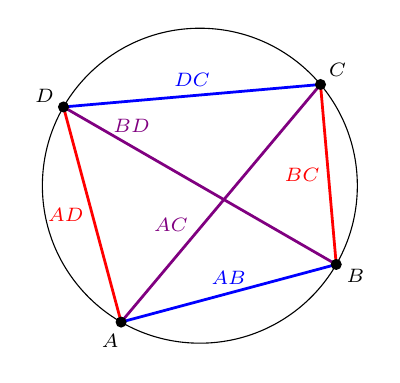
\begin{tikzpicture}
		\coordinate (center) at (0,0);
		\def\radius{2cm}
		\draw (center) circle[radius=\radius];

		% points on the circle
		\path (center) ++(-120:\radius) coordinate (A);
		\path (center) ++(-30:\radius) coordinate (B);
		\path (center) ++(40:\radius) coordinate (C);
		\path (center) ++(150:\radius) coordinate (D);

		\begin{scriptsize}
			% Chords
			\draw[color=red, line width=1pt] (A) -- node[left] {$AD$} (D);
			\draw[color=red, line width=1pt] (B) -- node[left] {$BC$} (C);
			\draw[color=blue, line width=1pt] (A) -- node[above] {$AB$} (B);
			\draw[color=blue, line width=1pt] (D) -- node[above] {$DC$} (C);
			\draw[color=violet, line width=1pt] (A) -- node[above=8pt, near start] {$AC$} (C);
			\draw[color=violet, line width=1pt] (D) -- node[above=2pt, near start] {$BD$} (B);

			% Draw the points over the chords
			\fill[black] (A) circle[radius=2pt] ++(-120:1em) node {$A$};
			\fill[black] (B) circle[radius=2pt] ++(-30:1em) node {$B$};
			\fill[black] (C) circle[radius=2pt] ++(40:1em) node {$C$};
			\fill[black] (D) circle[radius=2pt] ++(150:1em) node {$D$};

		\end{scriptsize}
	\end{tikzpicture}
	\caption{Ptolomy's theorem:
	${\color{violet} |AC| \cdot |BD|}
		= {\color{red} |AD|\cdot |BC|} + {\color{blue} |AB| \cdot |CD|}$.}
	\label{fig:ptolomy}
\end{figure}

\begin{example}\label{exmp:triangulations}

	Note that \cref{thm:ptolomy} allows one to compute the length of one of the diagonals
	in terms of the other, given the side lengths. We will now apply this to triangulations
	of polygons.

	Let $1, 2, \dots, n$ denote $n$ points on a circle, arranged in cyclic order. By
	connecting these points through sides $P_{i, i+1}$, where the indices are taken modulo
	$n$, we obtain a polygon with $n$-sides. A triangulation\index{triangulations!of
		polygons}, $T$, is a choice of $(n-3)$ non-crossing diagonals. This results in a
	partitioning of the polygon in $n-2$ triangles. We will see triangulations in much more
	detail in \cref{sec:triangulations_of_surfaces}, and will therefore keep things brief
	here. For now, it is enough to understand things visually (cf.
	\cref{fig:hexagon_triangulations}).
	\begin{figure}[ht]
		\centering

		\begin{tikzpicture}
			\node[name=h, shape=regular polygon, draw, regular polygon sides = 6, minimum size = 1.5cm]{};
			\draw[] (h.corner 1) -- (h.corner 3);
			\draw[] (h.corner 1) -- (h.corner 4);
			\draw[] (h.corner 1) -- (h.corner 5);
		\end{tikzpicture}
		\begin{tikzpicture}
			\node[name=h, shape=regular polygon, draw, regular polygon sides = 6, minimum size = 1.5cm]{};
			\draw[] (h.corner 2) -- (h.corner 5);
			\draw[] (h.corner 2) -- (h.corner 4);
			\draw[] (h.corner 1) -- (h.corner 5);
		\end{tikzpicture}
		\begin{tikzpicture}
			\node[name=h, shape=regular polygon, draw, regular polygon sides = 6, minimum size = 1.5cm]{};
			\draw[] (h.corner 1) -- (h.corner 3);
			\draw[] (h.corner 3) -- (h.corner 5);
			\draw[] (h.corner 1) -- (h.corner 5);
		\end{tikzpicture}
		\caption{The triangulations of a regular hexagon up to rotation.}
		\label{fig:hexagon_triangulations}
	\end{figure}

	Starting from a triangulation, $T$, we obtain a new triangulation, $T'$, by
	``flipping'' a diagonal. Any diagonal in a triangulation lies on precisely 2 triangles.
	These two triangles form a quadrilateral. To flip the diagonal, you replace it with the
	other diagonal of that quadrilateral. Again, this is most easily seen visually:
	\begin{equation*}
		\begin{tikzpicture}[baseline]
			\node[name=h, shape=regular polygon, draw, regular polygon sides = 6, minimum size = 1.5cm]{};
			\draw[] (h.corner 1) -- (h.corner 3);
			\draw[dashed] (h.corner 1) -- (h.corner 4);
			\draw[] (h.corner 1) -- (h.corner 5);
		\end{tikzpicture}
		\quad \leadsto \quad
		\begin{tikzpicture}[baseline]
			\node[name=h, shape=regular polygon, draw, regular polygon sides = 6, minimum size = 1.5cm]{};
			\draw[] (h.corner 1) -- (h.corner 3);
			\draw[dashed] (h.corner 3) -- (h.corner 5);
			\draw[] (h.corner 1) -- (h.corner 5);
		\end{tikzpicture}
	\end{equation*}
	%
	Using Ptolomy's theorem, the length of the new diagonal can be computed given that we
	knew the lengths of all the edges in the previous triangulation. We now ignore
	Euclidean geometry, and just use Ptolomy's theorem as a recurrence relation to
	construct a collection of numbers as follows. Pick a triangulation and set all the edge
	lengths equal to one. Then at each step, choose a diagonal in the triangulation and
	flip it. Compute its edge length using Ptolomy's theorem. This is the next number in
	the collection. For example, we could obtain a sequence starting like this (we omit the
	ones on the sides):
	\begin{equation*}
		\begin{tikzpicture}[baseline]
			\node[name=h, shape=regular polygon, draw, regular polygon sides = 6, minimum size = 1.5cm]{};
			\draw[] (h.corner 1) -- node[fill=white, font=\footnotesize] {1} (h.corner 3);
			\draw[] (h.corner 1) -- node[fill=white, font=\footnotesize] {1} (h.corner 4);
			\draw[] (h.corner 1) -- node[fill=white, font=\footnotesize] {1} (h.corner 5);
		\end{tikzpicture}
		\leadsto
		\begin{tikzpicture}[baseline]
			\node[name=h, shape=regular polygon, draw, regular polygon sides = 6, minimum size = 1.5cm]{};
			\draw[] (h.corner 1) -- node[fill=white, font=\footnotesize] {1} (h.corner 3);
			\draw[dashed] (h.corner 3) -- node[fill=white, font=\footnotesize] {2} (h.corner 5);
			\draw[] (h.corner 1) -- node[fill=white, font=\footnotesize] {1} (h.corner 5);
		\end{tikzpicture}
		\leadsto
		\begin{tikzpicture}[baseline]
			\node[name=h, shape=regular polygon, draw, regular polygon sides = 6, minimum size = 1.5cm]{};
			\draw[dashed] (h.corner 2) -- node[fill=white, font=\footnotesize] {3} (h.corner 5);
			\draw[] (h.corner 3) -- node[fill=white, font=\footnotesize] {2} (h.corner 5);
			\draw[] (h.corner 1) -- node[fill=white, font=\footnotesize] {1} (h.corner 5);
		\end{tikzpicture}
		\leadsto
		\begin{tikzpicture}[baseline]
			\node[name=h, shape=regular polygon, draw, regular polygon sides = 6, minimum size = 1.5cm]{};
			\draw[] (h.corner 2) -- node[fill=white, font=\footnotesize] {3} (h.corner 5);
			\draw[] (h.corner 3) -- node[fill=white, font=\footnotesize] {2} (h.corner 5);
			\draw[dashed] (h.corner 2) -- node[fill=white, font=\footnotesize] {4} (h.corner 6);
		\end{tikzpicture}
		\leadsto
		\begin{tikzpicture}[baseline]
			\node[name=h, shape=regular polygon, draw, regular polygon sides = 6, minimum size = 1.5cm]{};
			\draw[dashed] (h.corner 3) -- node[fill=white, font=\footnotesize] {3} (h.corner 6);
			\draw[] (h.corner 3) -- node[fill=white, font=\footnotesize] {2} (h.corner 5);
			\draw[] (h.corner 2) -- node[fill=white, font=\footnotesize] {4} (h.corner 6);
		\end{tikzpicture}
		\leadsto
		\begin{tikzpicture}[baseline]
			\node[name=h, shape=regular polygon, draw, regular polygon sides = 6, minimum size = 1.5cm]{};
			\draw[] (h.corner 3) -- node[fill=white, font=\footnotesize] {3} (h.corner 6);
			\draw[] (h.corner 3) -- node[fill=white, font=\footnotesize] {2} (h.corner 5);
			\draw[dashed] (h.corner 3) -- node[fill=white, font=\footnotesize] {1} (h.corner 1);
		\end{tikzpicture}
		\leadsto \cdots
	\end{equation*}
	%
	Once again, we observe that we only obtain integers. Furthermore, there seems to be a
	limit to which integers we can obtain this way. This hints at a hidden periodicity. The
	Laurent phenomenon offers an explanation for why we only obtain integers: the lengths
	of the diagonals are Laurent polynomials in the originally chosen lengths.
\end{example}

There are many more examples like the three that we just gave. One can look at wiring
diagrams, generalized Somos sequences, knight recurrence, the Gale-Robinson sequence,
etc. As the focus of this thesis is not on number theory, we refrain from delving
deeper into this interesting world. We refer interested readers to \cite[Chapter
	3.4]{FominWilliams2021IntroductionCA_1-3} and \cite{FominZelevinsky2002Laurent}.

\subsection{Quivers, seeds and mutations}\label{sec:quivers_seeds_mutations}

In the examples from \cref{sec:integer_sequences} we made a couple of observations. In
each case, the sequence consisted of positive integers, something which was not so
obvious from the initial definitions. For
\cref{exmp:frieze_patterns,exmp:triangulations}, we also found some form of finiteness
and periodicity. There are some more subtle similarities, which will be explained in
detail in \cref{sec:sequences_revisited}. Before that, we must introduce the notion of
a cluster algebra. These can be constructed from a quiver, as we now explain.

\begin{definition}[Quivers]

	A \emph{quiver}\index{quiver} is a finite directed (multi)-graph with no 1-cycles
	(vertex connected to itself) or 2-cycles (two vertices connected by a pair of opposite
	arrows) (cf. \cref{fig:quivers}). For a quiver $Q$, we will denote the set of vertices
	with $Q_0$\index{Q 0@$Q_0$}.
\end{definition}

\begin{figure}[ht!]
	\centering
	\begin{equation*}
		\begin{tikzcd}
			&\bullet \arrow[loop] \arrow[r] &\bullet \\
			\bullet \rar & \bullet \arrow[r, bend left] & \bullet \arrow[l, bend left]
		\end{tikzcd}
		\hspace{2cm}
		\begin{tikzcd}[row sep=small]
			&&& \bullet \\
			\bullet \ar[rrrd, bend right]\rar &\bullet  \rar[leftarrow] &\bullet \ar[ru, shift left] \ar[ru, shift right] \ar[rd] \\
			&&& \bullet\\
			\\
			\bullet \ar[rr] && \bullet \ar[ld]\\
			& \bullet \ar[lu]
		\end{tikzcd}
	\end{equation*}
	\caption{The graphs on the left are not quivers, the graphs on the right are.}
	\label{fig:quivers}
\end{figure}

Let us now fix some notation for what follows. Write $[a,b] = \{a, a + 1, \dots, b\}$
for integers $a,b \in \bbZ$, where $[a,b] = \emptyset$ if $a > b$. Fix an integer $N
	\in \bbZ_{\geq 0}$, and a field $\bbK$ of characteristic zero. Finally, let $\mcF =
	\bbK (Y_1, \dots, Y_N)$ be the \emph{field of rational functions}\index{rational
	function field} over $\bbK$, in $N$ variables. Thus, $\mcF$ consists of fractions $P/Q$
where $P, Q\in \bbK[Y_1, \dots, Y_N]$ are polynomials in the variables $Y_1, \dots,
	Y_N$, and $Q$ is non-zero. In most cases we will take $\bbK = \bbC$ or $\bbK = \bbQ$.
This does not impact the definitions that follow in a meaningful way.

\begin{definition}
	We call a pair $(Q, \bx)$ a \emph{labeled seed}\index{seed!labeled} in $\mcF$ if
	\begin{enumerate}
		\item $Q$ is a quiver with vertices $Q_0 = [1, N]$.
		\item $\bx = (x_1, \dots, x_N)$ is a \emph{free generating set} of $\mcF$. That is, $\bx$ is a tuple of $N$ algebraically independent elements that generate $\mcF$.
	\end{enumerate}
	The tuple $\bx$ will be referred to as the \emph{cluster}\index{cluster}. The elements of $\bx$ will be called \emph{cluster variables}\index{cluster!variable}.
\end{definition}
%
One can also talk about \emph{unlabeled seeds}\index{seed!unlabeled}. An unlabeled seed
is an equivalence class of labeled seeds which are equal up to a simultaneous
re-indexing of the quiver vertices and the cluster variables. We will not need
unlabeled seeds as much, and will hence adopt the following convention.
\begin{convention}
	From now on, when we say \emph{seed}, we will always mean a labeled seed.
\end{convention}

Just like in nature, a seed on it own is not so interesting. We are interested in what
one can obtain from the seed. From a given seed, we can make another seed through a
process known as \emph{seed mutation}\index{seed!mutation}.
\begin{definition}

	Let $k \in \ex$ be an exchangeable vertex of the quiver $Q$. We define the
	\emph{mutation in direction $k$} of the seed $(Q, \bx)$ to be the seed $\mu_k(Q, \bx)
		\defeq (Q', \bx') = (\mu_k(Q), \mu_k(\bx))$\index{mu k@$\mu_k$}, where
	\begin{enumerate}
		\item $Q'_0 \defeq Q_0$.
		\item For every pair of vertices $i,j$ with $s$ arrows $i \to k$ and $t$ arrows $k \to j$ we
		      ``collapse'' these arrows into $s\cdot t$ arrows $i \to j$, cancelling pairwise with
		      any arrows $j \to i$.
		      \begin{equation*}
			      \begin{tikzcd}[column sep=small]
				      i \ar[rr, "r"] \ar[rd, "s"] && j \\
				      & k \ar[ur, "t"]
			      \end{tikzcd}
			      \quad \begin{tikzcd}
				      \; \rar[rightsquigarrow, "\mu_k"]& \;
			      \end{tikzcd}\quad
			      \begin{tikzcd}[column sep=small]
				      i \ar[rr, "r + st"] \ar[rd,leftarrow, "s"] && j \\
				      & k \ar[ur, leftarrow, "t"]
			      \end{tikzcd}
		      \end{equation*}
		      Here we take $r$ to be negative, if the arrows actually point the other way, as the path $i \to k \to j$.
		\item All arrows in $Q$ starting or ending in $k$ get their orientation flipped.
		\item $\bx' = (x_1', \dots, x_N')$, where $x_i' = x_i$ for $i \neq k$, and $x'_k$
		      is given by the \emph{exchange relation}\index{exchange relation}
		      \begin{equation}\label{eq:exchange_relation_quiver}
			      x'_k \defeq \frac{1}{x_k} \left(\prod_{i \to k} x_i + \prod_{k \to j} x_j\right),
		      \end{equation}
		      where we take the product equal to 1 if $\{i \to k\} = \emptyset$ or $\{k \to j\} = \emptyset$.
	\end{enumerate}
\end{definition}

Let us first look at an example involving only the mutation of the quiver.
\begin{example}
	We mutate the given quiver at vertex 2:
	\begin{equation*}
		\begin{tikzcd}
			& 4 \dlar \rar & 6 \dar \\
			1 \rar & 2 \uar \rar \dar[shift left] \dar [shift right] & 5 \\
			& 3 \ular
		\end{tikzcd}
		\begin{tikzcd}
			\; \rar[rightsquigarrow, "\mu_2"] &\;
		\end{tikzcd}
		\begin{tikzcd}
			& 4 \rar \dar & 6 \dar \\
			1  \drar \ar[rr,controls = {+(1, -2) and +(-1, -2)}] & 2 \lar & 5 \lar \\
			& 3 \uar[shift right] \uar[shift left]
		\end{tikzcd}
	\end{equation*}
	%
	The arrow $1 \to 2$ combined with the arrow $2 \to 4$ introduces one new arrow $1 \to
		4$ which cancels out the existing arrow $4 \to 1$. The arrow $1 \to 2$ combines with
	the 2 arrows $2 \to 3$ to create 2 new arrows $1 \to 3$, one of which cancels out with
	the existing arrow $3 \to 1$. Finally, the arrow $1 \to 2$ combined with the arrow $2
		\to 5$ yields an arrow $1 \to 5$. The arrows starting or ending in the vertex 6 remain
	unchanged.
\end{example}

Before we give some examples of seed mutation, we prove a small lemma, which will also
be useful for the examples.
\begin{lemma}\label{lem:mutation_involution}
	Seed mutation at a fixed vertex is an \emph{involution}\index{involution}, i.e., $\mu_k \circ \mu_k = id$.
\end{lemma}

\begin{proof}
	We first show that the quiver remains unchanged. For arrows incident to $k$, the
	mutation reverses the orientation. So, applying it twice yields the same orientation.
	Now, the only other part of the quiver that changes is at pairs of vertices $i,j$ with
	$s$ arrows $i \to k$ and $t$ arrows $k \to j$. Applying a single mutation introduces
	$s\cdot t$ new arrows $i \to j$. When applying the mutation the second time, we now
	have $s$ arrows $k \to i$ and $t$ arrows $j \to k$, due to the orientation flip of the
	arrows incident to $k$. Consequently, the mutation introduces $s \cdot t$ arrows $j \to
		i$ which cancel out exactly the arrows from the first mutation.

	That the cluster variables remain unchanged is a simple calculation:
	\begin{align*}
		x_k''
		 & = \frac{1}{x_k'}\left(\prod_{k \to i}x_i' + \prod_{j \to k} x_j'\right)                                                \\
		 & = x_k \left(\prod_{i \to k} x_i + \prod_{k \to j}x_j\right)^{-1} \left(\prod_{k \to i}x_i + \prod_{j \to k} x_j\right) \\
		 & = x_k,
	\end{align*}
	where we use that the exchange rule is unchanged by an orientation flip of all the arrows.
\end{proof}

\begin{example}
	The simplest example is the seed $(Q, \bx)$ where $Q$ is the quiver consisting of a single vertex:
	\begin{equation*}
		Q = \begin{tikzcd}
			\bullet
		\end{tikzcd},
		\quad \bx = (x).
	\end{equation*}
	%
	Mutating at the only vertex gives
	\begin{equation*}
		Q = \begin{tikzcd}
			\bullet
		\end{tikzcd},
		\quad \bx = \left(\frac{2}{x}\right).
	\end{equation*}
	%
	If we mutate again, we end up with the original seed, as a consequence of
	\cref{lem:mutation_involution}. It is of course also straightforward to verify it
	directly.
\end{example}
\begin{example}\label{exmp:A2_quiver}
	The next simplest example is the $A_2$ quiver\index{quiver!$A_2$}:
	\begin{equation*}
		Q = \begin{tikzcd}
			1 \rar &2
		\end{tikzcd},
		\quad \bx = \left(x_1, x_2\right).
	\end{equation*}
	%
	If we apply a mutation at the first vertex, we obtain:
	\begin{equation*}
		\mu_1(Q) = \begin{tikzcd}
			1 & \lar 2
		\end{tikzcd},
		\quad \mu_1(\bx) = \left(\frac{1+x_2}{x_1}, x_2\right).
	\end{equation*}
	%
	We already know that mutating at the first vertex again will yield the same seed, so
	the only interesting thing to do is to see what happens after mutating at index 2:
	\begin{equation*}
		\mu_2(\mu_1(Q)) = \begin{tikzcd}
			1 \rar & 2
		\end{tikzcd},
		\quad  \mu_2(\mu_1(\bx)) = \left(\frac{1+x_2}{x_1}, \frac{x_1 + x_2 + 1}{x_1 x_2}\right).
	\end{equation*}
	%
	Although we are back at the original quiver, the cluster variables are completely
	different. We now mutate again at the first vertex. We will use the notation
	$\mu_{k_1k_2\cdots k_l}$ as a shorthand for $\mu_{k_l} \circ \cdots \circ \mu_{k_2}
		\circ \mu_{k_1}$.
	\begin{equation*}
		\mu_{121}(Q) = \begin{tikzcd}
			1 &\lar 2
		\end{tikzcd},
		\quad  \mu_{121}(\bx) = \left(\frac{x_1(x_1 x_2 + x_1 + x_2 + 1)}{x_1x_2(1+x_2)}, \frac{x_1 + x_2 + 1}{x_2}\right).
	\end{equation*}
	%
	The expression for the first cluster variable looks complicated, but can be
	dramatically simplified to $\frac{x_1 + 1}{x_2}$. We continue mutating:
	\begin{equation*}
		\mu_{1212}(Q) = \begin{tikzcd}
			1 \rar& 2
		\end{tikzcd},
		\quad  \mu_{1212}(\bx) = \left(\frac{x_1 + 1}{x_2}, x_1\right).
	\end{equation*}
	%
	Once again, some simplification has taken place. We mutate a final time at the first
	vertex.
	\begin{equation*}
		\mu_{12121}(Q) = \begin{tikzcd}
			1 &\lar 2
		\end{tikzcd},
		\quad  \mu_{12121}(\bx) = \left(x_2, x_1\right).
	\end{equation*}

	We have our original seed, except that the arrow in the quiver has been reversed, and
	that $x_1$ and $x_2$ have swapped places. In other words, after 5 mutations, the roles
	of 1 and 2 have swapped. It follows that another 5 swaps will give back the original
	seed.

	If one takes a close look at the obtained cluster variables, then we see that these
	correspond exactly to those that we found when trying to construct a frieze pattern
	with 2 rows (cf. \cref{exmp:frieze_patterns}). This is no coincidence, and we will come
	back to this in \cref{sec:sequences_revisited}.
\end{example}

\begin{example}
	The logical follow-up to the $A_2$ quiver is the $A_3$ quiver\index{quiver!$A_3$}
	\begin{equation*}
		Q =
		\begin{tikzcd}
			1 \rar[] & 2 \rar[] &3
		\end{tikzcd},
		\quad \bx = \left(x_1, x_2, x_3\right).
	\end{equation*}
	Mutation in direction 2 gives
	\begin{equation*}
		\mu_2(Q) =
		\begin{tikzcd}
			1 \rar[leftarrow] \ar[rr, bend right] & 2 \rar[leftarrow]& 3
		\end{tikzcd},
		\quad \mu_2(\bx) = \left(x_1, \frac{x_1 + x_3}{x_2}, x_3\right).
	\end{equation*}
	If we instead apply a mutation in direction 1, we find
	\begin{equation*}
		\mu_1(Q) =
		\begin{tikzcd}
			1 \rar[leftarrow] & 2 \rar[]& 3
		\end{tikzcd},
		\quad \mu_1(\bx) = \left(\frac{x_2 + 1}{x_1}, x_2, x_3\right).
	\end{equation*}
	Finally, a mutation in direction 3 would give
	\begin{equation*}
		\mu_3(Q) =
		\begin{tikzcd}
			1 \rar[] & 2 \rar[leftarrow]& 3
		\end{tikzcd},
		\quad \mu_3(\bx) = \left(x_1, x_2, \frac{x_2 + 1}{x_3}\right).
	\end{equation*}
	Mutating in direction 1 on $\mu_2(Q)$ gives
	\begin{equation*}
		\mu_{21}(Q) =
		\begin{tikzcd}
			1 \rar[] \ar[rr,leftarrow, bend right] & 2 & 3
		\end{tikzcd},
		\quad \mu_{21}(\bx) = \left(\frac{x_1 + x_3 + x_2x_3}{x_1x_2}, \frac{x_1 + x_3}{x_2}, x_3\right).
	\end{equation*}
	If we now mutate in direction 3, we obtain
	\begin{equation*}
		\mu_{213}(Q) =
		\begin{tikzcd}
			1 \rar[] \ar[rr, bend right] & 2 & 3
		\end{tikzcd},
		\quad \mu_{213}(\bx) = \left(\frac{x_1 + x_3 + x_2x_3}{x_1x_2}, \frac{x_1 + x_3}{x_2}, \frac{x_1 x_2 + x_1 + x_3 + x_2 x_3}{x_1x_2x_3}\right).
	\end{equation*}
	It seems that the expressions keep getting messier and messier. We mutate again in direction 2:
	\begin{equation*}
		\mu_{2132}(Q) =
		\begin{tikzcd}
			1 \rar[leftarrow] \ar[rr, bend right] & 2 & 3
		\end{tikzcd},
	\end{equation*}
	\begin{equation*}
		\mu_{2132}(\bx)= \left(\frac{x_1 + x_3 + x_2x_3}{x_1x_2}, \frac{x_2 + 1}{x_1}, \frac{x_1 x_2 + x_1 + x_3 + x_2 x_3}{x_1x_2x_3}\right).
	\end{equation*}
	Somehow, some miraculous cancelation happened.
	Note that the expression $\frac{x_2 + 1}{x_2}$ already appeared previously.
	If we instead mutate in direction 1, we get
	\begin{equation*}
		\mu_{2131}(Q) =
		\begin{tikzcd}
			1 \rar[leftarrow] \ar[rr,leftarrow, bend right] & 2 & 3
		\end{tikzcd},
	\end{equation*}
	\begin{equation*}
		\mu_{2131}(\bx) = \left(\frac{x_1 + x_3 + x_1x_2}{x_2x_3}, \frac{x_1 + x_3}{x_2}, \frac{x_1 x_2 + x_1 + x_3 + x_2 x_3}{x_1x_2x_3}\right).
	\end{equation*}
	This still introduces a new expression.
	Interestingly, these are all the possible expressions we can obtain!
	If we now mutate in, say, direction 3, we would get as cluster
	\begin{equation*}
		\mu_{21313} = \left(\frac{x_1 + x_3 + x_1x_2}{x_2x_3}, \frac{x_1 + x_3}{x_2}, x_1 \right).
	\end{equation*}
	This is again a dramatic cancelation. One can check manually
	that no mutations introduce new cluster variables.
\end{example}

\begin{example}\label{exmp:markov_quiver}
	As a last example, we look at the \emph{Markov quiver}\index{quiver!Markov}\index{Markov!quiver}:
	\begin{equation*}
		\begin{tikzcd}[column sep= small]
			& 1 \ar[ld, shift left] \ar[ld, shift right]\\
			2 \ar[rr, shift left] \ar[rr, shift right] && 3 \ar[lu, shift left] \ar[lu, shift right]
		\end{tikzcd},
	\end{equation*}
	%
	which possesses the special property that it remains invariant under mutations at any
	vertex (up to a simultaneous flipping of all the arrows). Let us see what happens to
	the cluster variables as we mutate in a cyclic order of the vertices. Denote for
	brevity $x \defeq x_1, y \defeq x_2$ and $z \defeq x_3$ for the cluster variables
	corresponding to the vertices $1,2$ and $3$ respectively. Because the exchange relation
	is invariant under a flipping of all the arrows and the Markov quiver is rotationally
	symmetric, the exchange relation will always be of the form
	\begin{equation}\label{eq:markov_exchange_relation}
		w' = \frac{u^2 + v^2}{w},
	\end{equation}
	%
	where $u, v$ and $w$ are the cluster variables of the seed being mutated. Thus, we
	obtain
	\begin{align*}
		\bx            & = \{x, y, z\}                                                                                                                                                                              \\
		\mu_1(\bx)     & = \left(\frac{y^2 + z^2}{x}, y, z\right)                                                                                                                                                   \\
		\mu_{12}(\bx)  & = \left(\frac{y^2 + z^2}{x}, \frac{y^4 + 2 z^2y^2 +z^4 + z^2x^2 }{x^2y}, z\right)                                                                                                          \\
		\mu_{123}(\bx) & = \left(\frac{y^2 + z^2}{x}, \frac{y^4 + 2 z^2y^2 +z^4 + z^2x^2 }{x^2y},\right.                                                                                                            \\
		               & \left. \frac{x^{4} z^{4} + x^{2} y^{6} + 4 x^{2} y^{4} z^{2} + 5 x^{2} y^{2} z^{4} + 2 x^{2} z^{6} + y^{8} + 4 y^{6} z^{2} + 6 y^{4} z^{4} + 4 y^{2} z^{6} + z^{8}}{x^{4} y^{2} z} \right)
	\end{align*}
	%
	Mutating again at the first vertex gives the new cluster variable
	\begin{align*}
		 & \frac{x^{8} z^{6} + 4 x^{6} y^{4} z^{4} + 8 x^{6} y^{2} z^{6} + 4 x^{6} z^{8} + x^{4} y^{10} + 8 x^{4} y^{8} z^{2} + 24 x^{4} y^{6} z^{4} + 34 x^{4} y^{4} z^{6} + 23 x^{4} y^{2} z^{8}}{x^7y^4z^2} \\&+ \frac{6 x^{4} z^{10} + 2 x^{2} y^{12} + 14 x^{2} y^{10} z^{2} + 40 x^{2} y^{8} z^{4} + 60 x^{2} y^{6} z^{6} + 50 x^{2} y^{4} z^{8} + 22 x^{2} y^{2} z^{10} + 4 x^{2} z^{12}}{x^7 y^4 z^2}\\ &+ \frac{y^{14} + 7 y^{12} z^{2} + 21 y^{10} z^{4} + 35 y^{8} z^{6} + 35 y^{6} z^{8} + 21 y^{4} z^{10} + 7 y^{2} z^{12} + z^{14}}{x^{7} y^{4} z^{2}}.
	\end{align*}
	%
	Because the author does not want to spend too much time fiddling with alignment points
	to get long fractions to fit on a page, we will stop here. Mutating at vertex 2 would
	yield another fraction with 65 terms (with positive integer coefficients) in the
	numerator, and the expression $x^{12}y^7z^4$ in the denominator.

	Unlike the previous examples, the cluster variables do not simplify. In fact, one can
	show, that the number of cluster variables is infinite (cf.
	\cref{thm:cluster_finite_classification}). This is in contrast to the quiver itself,
	whose only mutation corresponds to a reversal of all the arrows.
\end{example}

\subsection{The cluster algebra}

From the examples of \cref{sec:quivers_seeds_mutations} we gather the following
observations:
\begin{enumerate}
	\item Even though a sequence of mutations might result in the same quiver, the corresponding
	      cluster variables might be different.
	\item For some quivers, the number of obtainable cluster variables is finite.
	\item Independent of the quiver, all the cluster variables are Laurent polynomials in the
	      original cluster variables.
	\item The Laurent polynomials have coefficients in the positive integers.
\end{enumerate}

To have the correct setting to explain the above observations, we must introduce the
notion of a \emph{cluster algebra}\index{cluster!algebra}\index{algebra!cluster}. From
\cref{lem:mutation_involution} it follows that the process of applying mutations is
invertible. This means that we get a well-defined notion of
\emph{mutation-equivalence}\index{mutation!-equivalence} of seeds. Two seeds are
\emph{equivalent}\index{seed!equivalent} if one can be obtained from the other through
a sequence of mutations.
\begin{definition}

	Choose some \emph{initial seed}\index{seed!initial} $(Q, \bx)$. The \emph{cluster
		algebra} $\mcA (Q, \bx)$\index{A Q x@$\mcA(Q, \bx)$} is the subalgebra of $\mcF$
	generated by all cluster variables $\bx'$ for seeds $(Q', \bx')$ mutation-equivalent to
	the initial seed $(Q, \bx)$.
\end{definition}
\begin{remark}

	Note that the definition of the cluster algebra only depends on the equivalence class
	of a seed.
\end{remark}

The first two observations are about two notions of ``finiteness'' of cluster algebras.
When there are only finitely many mutation-equivalent quivers, we say that the cluster
algebra is \emph{mutation-finite}\index{mutation!-finite}. When there are only finitely
many cluster variables, we say that the cluster algebra is
\emph{cluster-finite}\index{cluster!-finite}\footnote{It is also common to say that a
	cluster algebra is of finite type instead of calling it cluster-finite.}.

Mutation-finite cluster algebras need not be cluster-finite. For example, the Markov
quiver (\cref{exmp:markov_quiver}) is mutation-finite but has infinitely many cluster
variables. The inverse implication is true. Any cluster-finite cluster algebra is
automatically also mutation-finite. Indeed, suppose that there are finitely many
cluster variables, but infinitely many distinct quivers. By the pigeonhole principle,
there is some cluster which appears in infinitely many seeds. Since there are only
finitely many variables in the cluster, one of them has to appear in an infinite number
of exchange rules, but that leads to infinitely many new cluster variables.

Remarkably, it is possible to classify the cluster- and mutation-finite cluster
algebras. To state the classification more precisely, the following lemma is useful:
\begin{lemma}

	Let $Q$ be an unoriented finite tree. Then any two orientations of $Q$ are
	mutation-equivalent through mutations at only sources and sinks. Recall that a
	\emph{source}\index{source} is a vertex such that all arrows incident to the vertex
	point away from the vertex, while a \emph{sink}\index{sink} is a vertex such that all
	incident arrows point to the vertex.
\end{lemma}

\begin{proof}
	We prove this by induction on the number of vertices in $Q$. When $Q$ consists of just a single vertex, there is nothing to prove. Now assume that the statement holds for any tree with $n$ vertices, and let $Q$ be an unoriented tree with $n+1$ vertices. Fix an orientation of $Q$, and let $Q'$ be another orientation of $Q$. Since $Q$ is a tree, it has a leaf $v$, (a vertex of degree 1). Performing a mutation at $v$ only flips the orientation of the single arrow connected to it. Furthermore, it is always a source or a sink.

	Now, consider the subgraph of $Q_v$ obtained by removing $v$ and the arrow connected to
	it. This is a tree with $n$ vertices, and we can hence transform it, by induction, to
	the orientation $Q'_v$ by only mutating at sources and sinks. Write $w$ for the other
	vertex connected to $v$ in $Q$. Applying the same mutations to $Q$ instead of $Q_v$
	would yield the desired orientation for all the arrows, except possibly the arrow
	between $v$ and $w$. This can be fixed by mutating a final time at $v$ if necessary.

	There is one other subtlety. When applying the mutations to $Q$ instead of $Q_v$, it is
	possible that $w$ would no longer be a source or sink due to the extra arrow between
	$v$ and $w$. This is easily amended by applying a mutation at $v$ whenever the
	orientation of the arrow between $v$ and $w$ is wrong.
\end{proof}

Some converse of this theorem is also true, but the proof is no longer purely
combinatorial, and requires advanced techniques:
\begin{theorem}[\cite{CalderoKeller2006TriangulatedCat}]

	Let $Q$ and $Q'$ be two acyclic quivers\index{quiver!acyclic} (without oriented cycles)
	which are mutation-equivalent. Then $Q$ can be transformed into $Q'$ via a sequence of
	mutations at sources and sinks. In particular, if an acyclic quiver is
	mutation-equivalent to an orientation of a tree, then it must be an orientation of the
	same tree. So, two non-isomorphic trees are never mutation-equivalent to each other.
\end{theorem}

We will state the classification theorem without proof, since it is interesting, but
not very relevant for the rest of the thesis. A complete proof can be found in, e.g.,
\cite{FominZelevinsky2003CAFin} or \cite{FominWilliams2021IntroductionCA_4-5}.
\begin{theorem}[Fomin--Zelevinsky]\label{thm:cluster_finite_classification}

	A cluster algebra $\mcA (Q, \bx)$ is cluster-finite if and only if each connected
	component of $Q$ is mutation-equivalent to a simply-laced, i.e., of type ADE, Dynkin
	diagram\index{Dynkin diagram} (cf. \cref{fig:dynkin_diagrams_ade}). In this case there
	is a bijective correspondence between the cluster variables and the almost positive
	roots $\Phi_{\geq -1}$, given by
	\begin{equation*}
		\alpha \leftrightarrow \frac{P_\alpha (\bx)}{x^\alpha},
	\end{equation*}
	where $P_\alpha (\bx)$ is a polynomial in $\bx$.
\end{theorem}

\begin{figure}[ht]
	\centering
	\begin{align*}
		 &
		\begin{aligned}
			 & A_n \quad \begin{tikzcd}[ampersand replacement=\&, sep=small]
				             \bullet \rar \& \bullet \rar \&\dots \rar \&\bullet
			             \end{tikzcd}               \\
			 & D_n \quad \begin{tikzcd}[ampersand replacement=\&, sep=small]
				             \&\&\&\&\bullet \\
				             \bullet \rar \& \bullet \rar \&\dots \rar \& \bullet \drar \urar \\
				             \&\&\&\&\bullet
			             \end{tikzcd}
		\end{aligned}
		 &   &
		\begin{aligned}
			 & E_6 \quad \begin{tikzcd}[ampersand replacement=\&, sep=small]
				             \&\&\bullet\\
				             \bullet \rar \& \bullet \rar \&\bullet \rar\uar \& \bullet \rar \& \bullet
			             \end{tikzcd}                                \\
			 & E_7 \quad \begin{tikzcd}[ampersand replacement=\&, sep=small]
				             \&\&\bullet\\
				             \bullet \rar \& \bullet \rar \&\bullet \rar\uar \& \bullet \rar \& \bullet \rar \& \bullet
			             \end{tikzcd}                \\
			 & E_8 \quad \begin{tikzcd}[ampersand replacement=\&, sep=small]
				             \&\&\bullet\\
				             \bullet \rar \& \bullet \rar \&\bullet \rar\uar \& \bullet \rar \& \bullet \rar \& \bullet\rar \& \bullet
			             \end{tikzcd}
		\end{aligned}
	\end{align*}

	\caption{The simply-laced Dynkin diagrams. They are indexed by the number of vertices.}
	\label{fig:dynkin_diagrams_ade}
\end{figure}

To understand the correspondence with the almost positive roots a bit better, we return
to the $A_3$ quiver. We obtained a total of $9 = 3 + 6$ cluster variables:
\begin{align*}
	 & x_1, x_2, x_3,                                                                                               \\
	 & \frac{x_2 + 1}{x_1}, \frac{x_1 + x_3}{x_2}, \frac{x_2 + 1}{x_3},                                             \\
	 & \frac{x_1+x_3+x_2x_3}{x_1x_2}, \frac{x_1+x_3+x_1x_2}{x_2x_3}, \frac{x_1x_2 + x_1 + x_3 + x_2x_3}{x_1x_2x_3}.
\end{align*}
%
We can write the positive roots of $A_3$ as $\{\alpha_1, \alpha_2, \alpha_3, \alpha_1 +
	\alpha_2, \alpha_2 + \alpha_3, \alpha_1 + \alpha_2 + \alpha_3\}$ for some choice of
simple roots $\alpha_1, \alpha_2, \alpha_3$. The simple roots correspond to the second
row of cluster variables, while the other positive roots correspond to the last row by
looking at the exponents in the denominator. In the theorem, one also includes the
additive inverses of the simple roots, i.e., $-\alpha_1, -\alpha_2, -\alpha_3$, such
that the original cluster variables are counted as well.

We already saw that cluster-finite cluster algebras are mutation-finite. Beyond those,
which other cluster algebras are mutation-finite? It turns out that, other than a few
exceptions, the only other ones are those originating from triangulations of surfaces
with boundary and punctures (which we will discuss in
\cref{sec:cluster_algebras_surfaces}) (\cite{FeliksonShapiroTumarkin2012SkewSCA}). An
example of a quiver that is not mutation-finite, is the following:
\begin{equation*}
	Q =
	\begin{tikzcd}[sep = small]
		& 3 & \\
		1 \urar &&2 \ular \\
		& 4 \ular \ar[uu] \urar
	\end{tikzcd}
\end{equation*}
%
After applying in order, the mutations at the vertices $1,2,3$ and 4, one obtains the
quivers
\begin{equation*}
	\mu_{1234}(Q) =
	\begin{tikzcd}[sep = small]
		& 3 & \\
		1 \urar[leftarrow, "5"] &&2 \ular[leftarrow, "5"'] \\
		& 4 \ular[leftarrow, "2"] \ar[uu, "3"] \urar[leftarrow, "2"']
	\end{tikzcd}
	,\quad \mu_{12341234}(Q) =
	\begin{tikzcd}[sep = small]
		& 3 & \\
		1 \urar["1406"] &&2 \ular["1406"'] \\
		& 4 \ular["83"] \ar[uu, "17"] \urar["83"']
	\end{tikzcd}
\end{equation*}
%
where the notation $\begin{tikzcd}[cramped, sep=small]
		a \ar[r, "r"] &b
	\end{tikzcd}$ indicates that there are $r$ arrows from vertex $a$ to vertex $b$. Repeating the same mutations will only increase the amount of arrows.

\medskip

Let us now look at the third and fourth observation that we made from the examples:
that all the cluster variables are Laurent polynomials with positive integer
coefficients, in the variables of the initial seed. At a first glance it might seem
obvious that all the coefficients would be positive, since the exchange rule does not
involve any subtractions. The subtlety comes from the cancelations that occur to reduce
the fractions to Laurent polynomials. For example, the fraction $\frac{x^3 +
		y^3}{x(x+y)}$ simplifies to $\frac{x^2 - xy + y^2}{x}$. We now formulate the much
alluded-to \emph{Laurent phenomenon}.
\begin{theorem}[Laurent Phenomenon\index{Laurent!-phenomenon}]\label{thm:laurent_phenomenon}

	Let $\mcA (Q, \bx)$ be a cluster algebra. Each of the cluster variables can be written
	as a Laurent polynomial in $\bx$ with integer coefficients.
\end{theorem}
%
This theorem was already proven by Fomin and Zelevinsky in their paper from 2002
introducing cluster algebras (\cite[Theorem 3.1]{FominZelevinsky2002CAF}). They
conjectured that all the coefficients would be positive. This remained an open
conjecture for quite some time, and was first proven by Lee and Schiffler in 2015 for
cluster algebras coming from quivers (\cite{LeeSchiffler2015PositivityCA}).

An alternative perspective on the Laurent phenomenon is given by looking at the
\emph{upper cluster algebra}\index{algebra!upper cluster}. Let $\mcA(Q, \bx)$ be a
cluster algebra, then the associated \emph{upper cluster algebra} is defined as the
$\mcF$-subalgebra
\begin{equation*}
	\mcU(Q, \bx) = \bigcap_{(Q', \bx')} \bbK[(x_1')^{\pm 1}, \dots, (x'_N)^{\pm 1}],
\end{equation*}
%
where the intersection is over all seeds mutation-equivalent to $(Q, \bx)$. In other
words, it is the $\mcF$-subalgebra consisting of all the elements which are Laurent
polynomials in the cluster variables of any seed mutation-equivalent to $(Q, \bx)$. The
Laurent phenomenon then implies that
\begin{equation*}
	\mcA(Q, \bx) \subseteq \mcU(Q, \bx).
\end{equation*}

An important question is to determine when $\mcA(Q, \bx) = \mcU(Q, \bx)$. This was
first studied by Berenstein, Fomin and Zelevinsky in
\cite{BerensteinFominZelevinsky2005CA3UpperBoundsDBC}. There they showed that if $Q$ is
\emph{acyclic}\index{quiver!acyclic}, i.e., it contains no oriented cycles, then
$\mcA(Q, \bx) = \mcU(Q, \bx)$. In particular, this holds for cluster-finite cluster
algebras. Greg Muller showed in a later paper that equality holds for so-called
\emph{locally acyclic cluster algbras}\index{algebra!locally acyclic cluster}
(\cite{Muller2013LocallyAcyclicCA}). In \cref{sec:cgl_extensions} we will study a broad
class of quantum cluster algebras for which equality between the quantum cluster
algebra and the quantum upper cluster algebra. We now look at an example were equality
does not hold.

\begin{example}
	Consider the cluster algebra $\mcA(Q, \bx)$ from \cref{exmp:markov_quiver}. We claim that $\mcA(Q, \bx) \subsetneq \mcU(Q, \bx)$. For any seed with cluster variables $x,y$ and $z$, the mutated cluster variables are given by
	\begin{align*}
		x' & = \frac{y^2 + z^2}{x} = y^2 x\inv + z^2 x\inv  \\
		y' & = \frac{x^2 + z^2}{y} = x^2 y\inv + z^2 y\inv  \\
		z' & = \frac{x^2 + y^2}{z} = x^2 z\inv + y^2 z\inv.
	\end{align*}
	%
	Note that mutated cluster variables are
	\emph{homogeneous}\index{homogeneous!polynomial} Laurent polynomials of degree one,
	i.e., all the monomials are of degree one, just like the original cluster variables.
	From this it follows that $\mcA(Q, \bx)$ is a $\bbZ_{\geq 0}$\emph{-graded
		algebra}\index{algebra!graded} such that all the cluster variables are homogeneous of
	degree one. Thus
	\begin{equation*}
		\mcA(Q, \bx) = \bigoplus_{n \in \bbZ_{\geq 0}} A_n,
	\end{equation*}
	%
	with $A_n A_m \subseteq A_{n+m}$, where $A_n \subseteq \mcA(Q, \bx)$ is the subset of
	all homogeneous Laurent polynomials of degree $n$.

	We now claim that
	\begin{equation*}
		w = \frac{x^2 + y^2 + z^2}{xyz} = xy\inv z\inv+ x\inv y z\inv + x\inv y \inv z \in \mcU(Q, \bx),
	\end{equation*}
	%
	which would show that $\mcU(Q, \bx) \neq \mcA(Q, \bx)$, since $w$ is homogeneous of
	degree $-1$. One way to prove this claim is to make use of \cite[Corollary
		1.7]{BerensteinFominZelevinsky2005CA3UpperBoundsDBC}, which when applied to this
	setting yields
	\begin{align*}
		\mcU(Q, \bx)
		 & = \bbK[\bx^{\pm 1}] \cap \bbK[(\mu_1(\bx))^{\pm 1}] \cap \bbK[(\mu_2(\bx))^{\pm 1}] \cap \bbK[(\mu_3(\bx))^{\pm 1}]                                       \\
		 & =
		\bbK[x^{\pm 1}, y^{\pm 1}, z^{\pm 1}] \cap \bbK[\left(\frac{y^2 + z^2}{x}\right)^{\pm 1}, y^{\pm 1}, z^{\pm 1}] \cap {}                                      \\
		 & \quad {}\cap\bbK[x^{\pm 1}, \left(\frac{x^2 + z^2}{y}\right)^{\pm 1}, z^{\pm 1}]\cap \bbK[x^{\pm 1},y^{\pm 1}, \left(\frac{x^2 + y^2}{z}\right)^{\pm 1}].
	\end{align*}
	Thus,
	\begin{equation*}
		\frac{x^2 + y^2 + z^2}{xyz} = xy\inv z\inv+ x\inv y z\inv + x\inv y \inv z \in \bbK[\bx^{\pm 1}],
	\end{equation*}
	and
	\begin{equation*}
		\frac{x^2 + y^2 + z^2}{xyz} = \frac{y^2 + z^2}{x}y\inv z\inv + (y^2  + z^2)\frac{x}{y^2 + z^2}y \inv z \inv \in \bbK[(\mu_1(\bx))^{\pm 1}].
	\end{equation*}
	The other cases follow by symmetry.

	A more direct approach is to show that $w$ is invariant under mutations. Indeed,
	\begin{align*}
		\frac{(\mu_1(x))^2 + (\mu_1(y))^2 + (\mu_1(z))^2}{\mu_1(x)\mu_1(y)\mu_1(z)}
		 & = \frac{\left(\frac{y^2 + z^2}{x}\right)^2 + y^2 + z^2}{\frac{y^2 + z^2}{x}yz} \\
		 & = \frac{\frac{y^2 + z^2}{x} + x}{yz}                                           \\
		 & = \frac{x^2 + y^2 + z^2}{xyz},
	\end{align*}
	%
	and the other cases follow by symmetry. Thus, since $w \in \bbK[\bx^{\pm 1}]$, we have
	$w \in \bbK[(\bx')^{\pm 1}]$ for any seed $(Q', \bx')$ mutation-equivalent to $(Q,
		\bx)$. Consequently, $w \in \mcU(Q, \bx)$. The invariance of $w$ under mutations should
	come as no surprise, since this is essentially what we showed when proving
	\cref{eq:markov_diophantine}.
\end{example}

\subsection{Integer sequences revisited}\label{sec:sequences_revisited}

We now revisit the examples from \cref{sec:integer_sequences} in the context of cluster
algebras. The theory of cluster algebras will provide convenient explanations for the
observations made. However, all the mentioned observations were already known long
before cluster algebras were invented.

\begin{example}

	As one might have guessed from the names, the sequence $(x_n)_{n \in \bbZ_{>0}}$ from
	\cref{exmp:markov_sequence} is related to the Markov quiver from
	\cref{exmp:markov_quiver}\index{Markov!quiver}. Let us call a triplet $(x,y,z) \in
		\bbZ_{> 0}^3$ a \emph{Markov triplet}\index{Markov!triplet} if it satisfies the Markov
	equation \cref{eq:markov_diophantine}:
	\begin{equation*}
		x^2 + y^2 + z^2 = 3 x y z.
	\end{equation*}
	%
	From \cref{exmp:markov_sequence} we know that any triple of consecutive elements in the
	sequence $(x_n)_{n \in \bbZ_{\geq 0}}$ satisfies the Markov equation. A consequence of
	the proof was that if $(x,y,z)$ is a Markov triplet, then so is
	\begin{equation*}
		(3 yz -x, y, z) = (\frac{y^2 + z^2}{x}, y, z).
	\end{equation*}
	%
	From the symmetry of the Markov equation, it follows that $(x, \frac{x^2 + z^2}{y}, z)$
	and $(x, y, \frac{x^2 + y^2}{z})$ are also Markov triplets. Comparing this to the
	exchange relation for the Markov quiver, \cref{eq:markov_exchange_relation}, we see
	that mutation sends Markov triplets to Markov triplets. The Laurent phenomenon now also
	provides an alternative proof that the sequence $(x_n)_{n\in \bbZ_{\geq 0}}$ consists
	only of integers. Indeed, since $x_0 = x_1 = x_2 = 1$, all the denominators are one,
	because they are monomials in the variables $x_0, x_1$ and $x_2$. Starting from the
	initial triplet $(1,1,1)$ and mutating in all possible directions yields
	\cref{fig:markov_exchange_graph}, where we identify triplets which are equal up to a
	permutation of the entries. Such graphs are known as \emph{exchange
		graphs}\index{exchange!graph}. The nodes consist of unlabeled seeds, and edges
	correspond to mutations.

	\begin{figure}[ht!]
		\centering
		\begin{tikzpicture}[
				scale = 0.8,
				x = 5pt,
				y = 2.3pt,
				%  V/.style = ,
				every edge quotes/.style = {auto,sloped,font=\footnotesize} ]
			% \begin{scope}[nodes=V]
			\node (0) at (0,0)  {$(1,1,1)$};
			\node (1) at (16,0)    {$(2,1,1)$};
			\node (12) at (32,0)          {$(2,5,1)$};
			%
			\node (121) at (48, 32)    {$(13,5,1)$};
			\node (1212)  at (64, 48) {$(13,34,1)$};
			\node (12121) at (85, 56) {$(89,34,1)$};
			\node (12123) at (85, 40) {$(13,34,1325)$};
			\node (1213)  at (64, 16) {$(13,5,194)$};
			\node (12131) at (85, 28) {$(2897,5,194)$};
			\node (12132) at (85, 8) {$(13,75961,194)$};
			%
			\node (123) at (48, -32)    {$(2,5,29)$};
			\node (1232)  at (64, -48) {$(2,169,29)$};
			\node (12323) at (85, -56) {$(2,169,985)$};
			\node (12321) at (85, -40) {$(14701,169,29)$};
			\node (1231)  at (64, -16) {$(433,5,29)$};
			\node (12313) at (85, -28) {$(433,5,6466)$};
			\node (12312) at (85, -8) {$(433,37666,29)$};
			% \end{scope}
			\draw   (0)  edge["$\mu_1$"] (1)
			(1)  edge["$\mu_2$"] (12)
			%
			(12)  edge["$\mu_1$"] (121)
			(121)  edge["$\mu_2$"] (1212)
			(1212)  edge["$\mu_1$"] (12121)
			(1212)  edge["$\mu_3$"] (12123)
			(121)  edge["$\mu_3$"] (1213)
			(1213)  edge["$\mu_1$"] (12131)
			(1213)  edge["$\mu_2$"] (12132)
			%
			(12)  edge["$\mu_3$"] (123)
			(123)  edge["$\mu_2$"] (1232)
			(1232)  edge["$\mu_1$"] (12321)
			(1232)  edge["$\mu_3$"] (12323)
			(123)  edge["$\mu_1$"] (1231)
			(1231)  edge["$\mu_3$"] (12313)
			(1231)  edge["$\mu_2$"] (12312)
			;
		\end{tikzpicture}

		\caption{A part of the exchange graph of the Markov quiver, where the nodes are labeled by the corresponding Markov triplet.}
		\label{fig:markov_exchange_graph}
	\end{figure}
\end{example}

\begin{example}

	The recurrence relation \cref{eq:somos_4}, defining the Somos-4 sequence\index{Somos-4
		sequence} can also be recovered from the seed mutations corresponding to a certain
	quiver. Namely, consider the seed
	\begin{equation*}
		Q =
		\begin{tikzcd}[sep=large]
			1 \drar[shift left] \drar[shift right] & 2 \lar \dlar[shift left] \dlar[shift right] \\
			4 \uar \rar & 3 \uar[shift left] \uar \uar[shift right]
		\end{tikzcd}
		,\quad
		\bx = ( x_1, x_2, x_3, x_4)
	\end{equation*}
	%
	Mutating at the first vertex gives the seed
	\begin{equation*}
		\mu_1(Q) =
		\begin{tikzcd}[sep=large]
			1 \dar \rar & 2 \dlar[shift left] \dlar[shift right]  \\
			4 \rar[shift left] \rar[shift right] \rar & 3 \uar \ular[shift left] \ular[shift right]
		\end{tikzcd}
		,\quad
		\mu_1(\bx) = \left( \frac{x_2 x_4 + x_3^2}{x_1}, x_2, x_3, x_4\right)
	\end{equation*}
	%
	We now note that $\mu_1(Q)$ is given by relabeling the vertices of $Q$ via $1 \mapsto
		2, 2 \mapsto 3, 3 \mapsto 4, 4\mapsto 1$, and that $\mu_1(x_1)$ is given by the same
	formula as \cref{eq:somos_4}. Thus, by mutating consecutively at the vertices
	$1,2,3,4,1,2,3,4,\dots$ the new cluster variables will correspond to the terms in the
	Somos-4 sequence. The Laurent phenomenon now guarantees that the sequence consists of
	integers when we set $a_0 = a_1 = a_2 = a_3 = 1$, as the denominators of all the terms
	will be monomials in $a_0, a_1, a_2$ and $a_3$.
\end{example}

\begin{example}

	We already gave an idea of how the Laurent phenomenon can be used to construct frieze
	patterns in \cref{exmp:frieze_patterns}\index{frieze pattern}. We can now make this
	more precise. Namely, to make a frieze pattern with $n$ rows (excluding the bounding
	rows of ones and zeros), one should consider the $A_n$ quiver (cf.
	\cref{fig:dynkin_diagrams_ade}). It will be easiest to explain this with an example.
	Consider again the frieze pattern:
	\begin{equation*}
		\dots\quad
		\begin{tikzcd}[
				sep = 0.2em, cramped,
			]
			1&&1&&1&&1&&1&&1&&1&&1&&1&&1&&1\\
			&1&&2&&2&&3&&1&&2&&4&&1&&2&&2&&3\\
			3&&1&&3&&5&&2&&1&&7&&3&&1&&3&&5\\
			&2&&1&&7&&3&&1&&3&&5&&2&&1&&7&&3\\
			3&&1&&2&&4&&1&&2&&2&&3&&1&&2&&4\\
			&1&&1&&1&&1&&1&&1&&1&&1&&1&&1&&1
		\end{tikzcd}
		\quad
		\dots
	\end{equation*}
	%
	In this case we need (an orientation of) the $A_4$ quiver. We can choose any lattice
	path from top to bottom. Then, the edges are oriented so that they always point from
	left to right.
	\begin{equation*}
		\dots\quad
		\begin{tikzcd}[
				sep = 0.2em, cramped,
			]
			1&&1&&1&&1&&1&&1&&1&&1&&1&&1&&1\\
			&1&&2&&2\drar[shorten=-0.15em] &&3&&1&&2&&4&&1&&2&&2&&3\\
			3&&1&&3&&5 \drar[shorten=-0.15em] &&2&&1&&7&&3&&1&&3&&5\\
			&2&&1&&7&&3&&1&&3&&5&&2&&1&&7&&3\\
			3&&1&&2&&4\urar[shorten=-0.15em] &&1&&2&&2&&3&&1&&2&&4\\
			&1&&1&&1&&1&&1&&1&&1&&1&&1&&1&&1
		\end{tikzcd}
		\quad
		\dots
	\end{equation*}
	%
	Mutating at a sink or a source, only changes the orientation of the edges, and does not
	introduce new edges. For example, mutation at a sink gives
	\begin{equation*}
		\begin{tikzcd}
			\cdots b \rar &d & \lar c \cdots & \, \rar[rightsquigarrow, "\mu_d"] & \,&
			\cdots  b & \lar \rar d & c \cdots
		\end{tikzcd}
	\end{equation*}
	%
	The mutated cluster variable corresponding to $d$ is then given by $d' = \frac{bc +
			1}{d}$. If we call this $a$, then find that $ad - bc = 1$, which is precisely the
	$\SL_2(\bbZ)$ diamond rule. Similarly, mutation at a source would compute $d$ in terms
	of $a$ in the $\SL_2(\bbZ)$ diamond. In the example, mutation at the vertex labeled 3
	results in changing the lattice path from $2 \to 5 \to 3 \gets 4$ to $2 \to 5 \gets 7
		\to 4$. Applying the Laurent phenomenon now shows that all the entries in the frieze
	pattern are Laurent polynomials in the entries of the initial lattice path. In
	particular, if one starts with a lattice path consisting of only ones, then all the
	entries will be integers. Do note that there exist frieze patterns which do not have a
	lattice path from top to bottom consisting of only ones:
	\begin{equation*}
		\begin{tikzcd}[sep=0.2em,cramped]
			1&&1&&1&&1&&1&&1&&1&&1&&1&&1&&1\\
			&1&&2&&4&&1&&2&&4&&1&&2&&4&&1&&2\\
			3&&1&&7&&3&&1&&7&&3&&1&&7&&3&&1\\
			&2&&3&&5&&2&&3&&5&&2&&3&&5&&2&&3\\
			3&&5&&2&&3&&5&&2&&3&&5&&2&&3&&5\\
			&7&&3&&1&&7&&3&&1&&7&&3&&1&&7&&3\\
			2&&4&&1&&2&&4&&1&&2&&4&&1&&2&&4\\
			&1&&1&&1&&1&&1&&1&&1&&1&&1&&1&&1
		\end{tikzcd}
	\end{equation*}

	The periodicity of the frieze patterns can also be explained through cluster algebras.
	It follows in part from \cref{thm:cluster_finite_classification}. A more precise
	conclusion about the periodicity can be obtained using more advanced results. For
	example, \cite[Theorem 8.8]{FominZelevinsky2007CA4Coefficients} gives that the period
	divides $2(n + 1 + 2) = 2n +6$. Indeed, in the frieze pattern of
	\cref{exmp:frieze_patterns} we had observed a period of $7$ which is exactly half of
	$2\cdot 4 + 6 = 14$. For a more detailed overview of the connections between cluster
	algebras and frieze patterns, we refer the reader to the survey paper
	\cite{BaurFaberGratz2018ConwayCoxeterFriezes}.
\end{example}

For \cref{exmp:triangulations} it will be more convenient to use a more general
definition of a cluster algebra. Namely, that of a cluster algebra with coefficients.

\section{Ice quivers and coefficients}\label{sec:ice_quivers_and_coefficients}

In the previous section we looked at cluster algebras coming from quivers. These are in
some sense the simplest kind of cluster algebras. In some cases, a more general notion
is needed. For example \cref{exmp:triangulations} will involve quivers with certain
vertices being frozen. When looking at quantum cluster algebras, we will need
skew-symmetrizable cluster algebras. All of these will be looked at in this section. To
avoid confusion, we will be very precise in this chapter with the names and
definitions. In the notation of this section, the cluster algebras coming from quivers
that we saw in the previous chapter would be referred to as a \emph{skew-symmetric
	cluster algebras of geometric type without coefficients}. Along the way, we will remove
more and more adjectives until we are just left with the definition of a cluster
algebra.

\subsection{Ice quivers}

Recall that in \cref{exmp:triangulations}, the length of a diagonal was obtained using
Ptolomy's theorem. The calculation involves the lengths of some of the diagonals, as
well as the lengths of some of the sides. Thus, the cluster variables should be
associated with both the diagonals as well as the sides. This poses a slight problem.
It is not possible to perform a flip on one of the sides of the $n$-gon. To fix this,
we will make a distinction between \emph{exchangeable} and \emph{frozen} vertices. This
leads to the notion of an \emph{ice quiver}\index{quiver!ice}.

Fix a subset $\ex \subseteq [1, N]$. The elements of $\ex$ will be called
\emph{exchangeable}\index{exchangeable}, while the elements of $\frz = [1, N] \setminus
	\ex$ will be called \emph{frozen}\index{frozen}. An \emph{ice quiver}, $\tQ$, is then
just the same as a normal quiver, except that we distinguish between the frozen and
exchangeable vertices. Although not strictly necessary, we will assume that the quiver
$\tQ$ contains no arrows between the frozen vertices, i.e., the vertices in $\tQ_0 \cap
	\frz$. Arrows between exchangeable and frozen vertices are allowed. When drawing a
quiver, the frozen vertices will be drawn with a box, while the exchangeable vertices
will just be drawn normally. The subquiver spanned by the exchangeable vertices, will
be called the \emph{principal part}\index{quiver!principal part of} of $\tQ$, and
denoted with just $Q$.

The definition of a seed remains very similar in this context. The naming will become
clear later.
\begin{definition}

	A \emph{skew-symmetric labeled seed of geometric type}\index{seed!skew-symmetric of
		geometric type} in $\mcF$ is a tuple $(\tQ, \tbx)$, where $\tQ$ is an ice quiver, and
	$\tbx = (x_1, \dots, x_N)$ is a free generating set of $\mcF$. The tuple $\tbx$ will be
	referred to as the \emph{extended cluster}\index{cluster!extended}, while the tuple
	$\bx = (x_i \in \tbx \mid i \in \ex)$ will be called the \emph{cluster}. The elements
	of $\bx$ will be called \emph{cluster variables}\index{cluster!variable}, while the
	elements of $\tbx \setminus \bx$ will be called \emph{frozen variables}.
\end{definition}

A seed such as in the previous section will be referred to as a \emph{skew-symmetric
	labeled seed of geometric type without coefficients}. It corresponds to the special
case where $\frz = \emptyset$. In the literature, the suffix ``with coefficients'' is
sometimes appended to indicate that $\frz \neq \emptyset$.

Seed mutation is now defined analogously, except that mutation can only be done at the
exchangeable indices, and that potential new arrows between frozen vertices in the ice
quiver are discarded. We then obtain the following definition.
\begin{definition}

	Let $\binv \subseteq \frz$ be any subset and $(\tQ, \tbx)$ be a skew-symmetric labeled
	seed of geometric type in $\mcF$. Write $R = \bbK[x_i, x_j^{\pm 1} \mid i \in \frz
		\setminus \binv,\, j \in \binv]$. Then the \emph{skew-symmetric cluster algebra of
		geometric type}\index{skew-symmetric!cluster algebra of geometric type}, $\mcA(\tQ,
		\tbx, \binv)$\index{A Qt xt inv@$\mcA(\tQ, \tbx, \binv)$} is the $R$-subalgebra of
	$\mcF$ generated by all the cluster variables of all the clusters of seeds
	mutation-equivalent to $(\tQ, \tbx)$.
\end{definition}

The main theorems from the previous section carry over with some small modifications.
\begin{theorem}

	Let $\mcA(\tQ, \tbx, \binv)$ be a skew-symmetric cluster algebra of geometric type.
	\begin{itemize}
		\item It is cluster-finite if and only if the ice quiver $\tQ$ is mutation-equivalent to an
		      ice quiver such that the connected components of its principal part are simply-laced
		      Dynkin diagrams \cite{FominZelevinsky2003CAFin}.
		\item It is mutation-finite if and only if it is either cluster-finite, obtained from a
		      surface or is one of a few exceptions \cite{FeliksonPavel2023cluster}.
		\item The Laurent phenomenon holds. More precisely, let $(\tQ', \tbx')$ be any seed
		      mutation-equivalent to $(\tQ, \tbx)$, and $x$ any cluster variable of this seed. Then
		      $x$ is a Laurent polynomial with integer coefficients in the extended cluster variables
		      of the initial seed \cite{FominZelevinsky2002CAF}. The frozen variables do not appear
		      as denominators in the Laurent polynomials, i.e., $x \in \bbZ[x_i^{\pm 1}, x_j \mid i
			      \in \ex,\, j \in \frz]$ \cite[Theorem 3.3.6]{FominWilliams2021IntroductionCA_1-3}.
		\item The integer coefficients can be taken to be positive
		      (\cite{LeeSchiffler2015PositivityCA}).
	\end{itemize}
\end{theorem}

\textbf{TODO: triangulations example revisited.}

\subsection{Skew-symmetrizable matrices}

Thusfar, all the cluster algebras have been constructed from (ice) quivers.
Equivalently, one can work with matrices, as we know explain.

Let $\tQ$ be an ice quiver with exchangeable vertices labeled by $\ex$ and frozen
vertices labeled by $\frz$. Associated to $\tQ$ is an $N \times |\ex|$ integer matrix
$(b_{ik}) = \tB \in M_{N \times \ex}(\bbZ)$. The notation indicates that the columns
are indexed by $\ex$ instead of $[1, |\ex|]$. The elements are given by
\begin{equation*}
	b_{ik} = \begin{dcases*}
		|\{ i \to k\}|, & if $\{i \to k\} \neq \emptyset$ \\
		-|\{k \to i\}|, & if $\{k \to i\} \neq \emptyset$ \\
		0,              & otherwise,
	\end{dcases*}
\end{equation*}
%
for $i \in [1, N]$ and $k \in \ex$. It is not a square matrix because we assume that
there are no arrows between frozen vertices. The $|\ex| \times |\ex|$ submatrix $B \in
	M_{\ex \times \ex}(\bbZ)$ of $\tB$ given by the rows in $\ex$ will be called the
\emph{principal part}\index{principal part} of $\tB$. Note that the principal part of
$\tB$ is \emph{skew-symmetric}\index{skew-symmetric}\index{matrix!skew-symmetric},
i.e., $b_{ik} = - b_{ki}$ for all $i,k \in \ex$ or equivalently $B^T = - B$.

Conversely, starting from a matrix $\tB \in M_{N \times \ex}(\bbZ)$ whose principal
part is skew-symmetric, one can associate an ice quiver $\tQ$, by placing $b_{ik}$
arrows from the vertex $i$ to the vertex $k$, for each $i \in [1, N]$ and $k \in \ex$.

\begin{example}
	Consider the ice quiver
	\begin{equation*}
		Q = \begin{tikzcd}[sep=scriptsize]
			\boxed{1} \\
			2 \uar \rar[shift left]\rar[shift right] & 3  \rar \dar & 4 \\
			& \boxed{5} \ular
		\end{tikzcd},
	\end{equation*}
	%
	where $\ex = \{2,3,4\}$. The associated matrix $\tB \in M_{5 \times \ex}$ and principal
	part $B \in M_{\ex \times \ex}$ are given by
	\begin{equation*}
		\tB =
		\begin{pmatrix}
			-1 & 0  & 0 \\
			0  & 2  & 0 \\
			-2 & 0  & 1 \\
			0  & -1 & 0 \\
			1  & -1 & 0
		\end{pmatrix}
		,\quad B =
		\begin{pmatrix}
			0  & 2  & 0 \\
			-2 & 0  & 1 \\
			0  & -1 & 0
		\end{pmatrix}.
	\end{equation*}
\end{example}

Let $\tQ$ be an ice quiver with associated matrix $\tB$. We now want to describe what
happens to the matrix $\tB$ after mutation. Take some $k \in \ex$, and denote the
elements of $\mu_k(\tB)$ with $b'_{ij}$.
\begin{enumerate}
	\item The vertices of $\tQ$ remain unchanged under mutation. Thus, $\mu_k(\tB) \in M_{N
				      \times \ex}(\bbZ)$.
	\item For $i \in [1, N]$ and $j \in \ex$, we need to create a new arrow $i \to j$ for each
	      path $i \to k \to j$. There is a path $i \to k \to j$ if and only if $b_{ik} >0$ and
	      $b_{kj} > 0$. The number of paths $i\to j\to k$ is then given by $b_{ik}b_{kj}$.
	      Conversely, we need to create an arrow $j \to i$ for each path $j \to k \to i$. Such
	      paths exist if $b_{ik} <0$ and $b_{kj} < 0$. In this case, the number of paths is also
	      given by $b_{ik}b_{kj}$.
	\item Finally, for $i \in [1,N]$, we need to flip the orientation of all the arrows $i \to k$
	      or $k \to i$. This translates to setting $b'_{ij} = -b_{ij}$ for all $i \in [1, N]$ and
	      $j \in \ex$ such that $i = k$ or $j = k$.
\end{enumerate}
As a result we derive the following mutation rule for the mutation in direction $k\in \ex$:
\begin{equation}\label{eq:mutation_rule_matrix_expanded}
	b'_{ij} \defeq \begin{dcases*}
		-b_{ij},               & if $i = k$ or $j = k$  \\
		b_{ij} + b_{ik}b_{kj}, & if $b_{ik},b_{kj} > 0$ \\
		b_{ij} - b_{ik}b_{kj}, & if $b_{ik},b_{kj} < 0$ \\
		b_{ij},                & otherwise,
	\end{dcases*}
	\quad \text{for } i \in [1, N],\,j \in \ex.
\end{equation}
%
This can be further condensed into the following rule.
\begin{equation}\label{eq:mutation_rule_matrix_condensed}
	b'_{ij} \defeq \begin{dcases*}
		-b_{ij},                                            & if $i = k$ or $j = k$ \\
		b_{ij} + \frac{|b_{ik}|b_{kj} + b_{ik}|b_{kj}|}{2}, & otherwise.
	\end{dcases*}
\end{equation}

To express the exchange relation in terms of the matrix $\tB$ we first introduce some
notation. Write $[b_{ij}]_{+} \defeq \max\{b_{ij}, 0\}$ and $[b_{ij}]_{-} \defeq
	\min\{b_{ij}, 0\}$. Then the exchange rule \cref{eq:exchange_relation_quiver}
translates into
\begin{equation}\label{eq:exchange_relation_matrix}
	x'_k = \frac{1}{x_k}\left(\prod_{i=1}^N x_i^{[b_{ik}]_{+}} + \prod_{i=1}^{N} x_i^{-[b_{ik}]_{-}}\right).
\end{equation}

Because working with the matrix $\tB$ is equivalent to working with the ice quiver
$\tQ$, we will use the same name for the corresponding seeds and cluster algebras.
\begin{definition}

	A \emph{skew-symmetric labeled seed of geometric type}\index{seed!skew-symmetric of
		geometric type} in $\mcF$ if a tuple $(\tB, \tbx)$, where $\tB \in M_{N \times
				\ex}(\bbZ)$ has skew-symmetric principal part, and $\tbx = (x_1, \dots, x_N)$ is a free
	generating set of $\mcF$. The principal part $B$ of $\tB$ will be called the
	\emph{exchange matrix}\index{matrix!exchange}, while $\tB$ will be referred to as the
	\emph{extended exchange matrix}\index{matrix!extended exchange}.

	The mutation of the seed $(\tB, \tbx)$ in direction $k \in \ex$ is given by the seed
	$(\mu_k(\tB), \mu_k(\tbx))$ where $\mu_k(\tB)$ is given by
	\cref{eq:mutation_rule_matrix_condensed} and $\mu_k(\tbx)$ is given by $(x_1', \dots,
		x_N')$ where $x_i' = x_i$ for $i\neq k$ and $x'_k$ is given by
	\cref{eq:exchange_relation_matrix}. The \emph{skew-symmetric cluster algebra of
		geometric type}\index{skew-symmetric!cluster algebra of geometric type}, $\mcA(\tB,
		\ex, \binv)$\index{A Bt xt inv@$\mcA(\tB, \tbx, \binv)$} is then defined completely
	analogously to the version with ice quivers.
\end{definition}

Interestingly, note that for \emph{any} matrix $\tB \in M_{N\times \ex}(\bbZ)$, the
mutation rule \cref{eq:mutation_rule_matrix_expanded}, defines an involution. Indeed,
if $i = k$ or $j = k$ then $b''_{ij} = -b'_{ij} = b_{ij}$. Otherwise, if $b_{ik} > 0$
and $b_{kj} >0$, then $b'_{ik} = -b_{ik} < 0$ and $b'_{kj} = -b_{kj} < 0$ so that
\begin{equation*}
	b''_{ij} = b'_{ij} - b'_{ik}b'_{kj} = b_{ij} + b_{ik}b_{kj} - b_{ik}b_{kj} = b_{ij}.
\end{equation*}
%
Similarly, if $b_{ik} < 0$ and $b_{kj} < 0$. In the other cases mutation does not
change $b_{ij}$.

Additionally, remark that if $B$ is the principal part of $\tB$, then the principal
part of $\mu_k(\tB)$ is given by $\mu_k(B)$. Thus, the mutation of $B$ does not depend
on the entries of $\tB$ which are not contained in $B$.

One might wonder if we can simply drop the skew-symmetric condition on the principal
part of $\tB$ all together. It turns out that in order to have a nice enough ``exchange
pattern'', the minimal requirement is that the principal part of $\tB$ and all matrices
mutation-equivalent to it should be \emph{sign-
	skew-symmetric}\index{skew-symmetric!sign-}\index{matrix!sign-skew-symmetric}
(\cite[Proposition 4.3]{FominZelevinsky2002CAF}). A matrix $B \in M_N(\bbZ)$ is said to
be sign-skew-symmetric if for all $i,j \in [1, N]$, the entries $b_{ij}$ and $b_{ji}$
are both zero, or have opposite signs. In particular, skew-symmetric matrices are sign
skew-symmetric. The problem is that mutation of a sign-skew-symmetric matrix might
yield a matrix which is no longer sign-skew-symmetric.

\begin{example}
	Consider the sign-skew-symmetric matrix
	\begin{equation*}
		C = \begin{pmatrix}
			0  & 1  & -1 \\
			-2 & 0  & 4  \\
			3  & -1 & 0
		\end{pmatrix}.
	\end{equation*}
	%
	Mutation in direction $1$ using \cref{eq:mutation_rule_matrix_expanded} gives the
	matrix
	\begin{equation*}
		\mu_1(C) = \begin{pmatrix}
			0  & -1 & 1 \\
			2  & 0  & 2 \\
			-3 & 2  & 0
		\end{pmatrix},
	\end{equation*}
	which is no longer sign-skew-symmetric.
\end{example}

There is a class of matrices between sign-skew-symmetric matrices and skew-symmetric
matrices. These are the \emph{skew-symmetrizable
	matrices}\index{matrix!skew-symmetrizable}. A matrix $B \in M_N(\bbZ)$ is said to be
skew-symmetrizable if there exist $d_1, \dots, d_N \in \bbZ_{\geq 0}$ such that
\begin{equation}\label{eq:skew_symmetrizable}
	d_i b_{ij} = -d_j b_{ji}\quad  \text{ for all } i,j \in [1, N].
\end{equation}
%
We say that $B$ is skew-symmetrizable by the integers $d_1, \dots, d_N$. Write $D \in
	M_N{\bbZ}$ for the diagonal matrix with the elements $d_1, \dots, d_N$ on the diagonal.
Then \cref{eq:skew_symmetrizable} translates to $(DB)^T = -DB$, i.e., the matrix $DB$
is skew-symmetric.

\begin{proposition}\label{prop:mutation_preserves_skew_symmetrizable}
	Suppose that $B \in M_N(\bbZ)$ is skew-symmetrizable by the positive integers $d_1, \dots, d_N \in \bbZ_{>0}$. Then $B$ is sign-skew-symmetric, and for any $k \in [1, N]$, the matrix $\mu_k(B)$ is sign-skew-symmetric and skew-symmetrizable by the same integers.
\end{proposition}
\begin{proof}
	Since the integers $d_1, \dots, d_N$ are strictly positive, \cref{eq:skew_symmetrizable} implies that $B$ is sign-skew-symmetric. Furthermore, for $i,j \in [1, N]$ we have
	\begin{equation*}
		d_i b'_{ij} = - d_i  b_{ij} = d_j b_{ji} = -d_j b'_{ji}
	\end{equation*}
	if $i =k$ or $j = k$, and
	\begin{align*}
		d_i b'_{ij}
		 & = d_i b_{ij} + \frac{|d_i b_{ik}|b_{kj} + d_i b_{ik}|b_{kj}|}{2}         \\
		 & = - d_j b_{ji} + \frac{|d_k b_{ki}|b_{kj} - d_k b_{ki}|b_{kj}|}{2}       \\
		 & = - d_j b_{ji} + \frac{ - |b_{ki}| d_j b_{jk} - b_{ki}|d_jb_{jk}|}{2}    \\
		 & = - d_j\left( b_{ji} + \frac{|b_{jk}|b_{ki} +  b_{jk}|b_{ki}|}{2}\right) \\
		 & = - d_jb'_{ji},
	\end{align*}
	otherwise.
\end{proof}

It is now a natural question to ask whether all sign-skew-symmetric matrices which
remain sign-skew-symmetric under mutations are skew-symmetrizable. This turns out not
to be the case. For example, for $\alpha, \beta, \gamma \in \bbZ_{>0}$ such that
$\alpha\beta\gamma \geq 0$, the matrix
\begin{equation*}
	\begin{pmatrix}
		0             & 2\alpha         & -2\alpha \beta \\
		-\beta \gamma & 0               & 2 \beta        \\
		\gamma        & - \alpha \gamma & 0
	\end{pmatrix}
\end{equation*}
%
is sign-skew-symmetric, not skew-symmetrizable, and it remains sign-skew-symmetric
under any sequence of mutations (\cite[Proposition 4.7]{FominZelevinsky2002CAF}). In
practice, however, one always restricts to the skew-symmetric or skew-symmetrizable
case.
\begin{definition}\label{def:cluster_algebra_geometric_type}

	A pair $(\tB, \tbx)$, where $\tB \in M_{N \times \ex}(\bbZ)$ is such that its principal
	part is skew-symmetrizable and $\tbx = (x_1, \dots, x_N)$ is a free generating set of
	$\mcF$ is called a \emph{labeled seed of geometric type}\index{seed!of geometric type}
	in $\mcF$. Seed mutation and the corresponding \emph{cluster algebra of geometric
		type}\index{cluster algebra!of geometric type} are defined completely analogously as in
	the case of skew-symmetric seeds of geometric type.
\end{definition}

The main results from the skew-symmetric case also hold in the skew-symmetrizable case.
The cluster-finite classification now encompasses all the Dynkin diagrams. We refer the
reader to \cite[Chapter 5]{FominWilliams2021IntroductionCA_4-5} for a good overview of
Cartan matrices, Dynkin diagrams and the classification.
\begin{theorem}[\protect{\cite[Theorem 1.4]{FominZelevinsky2003CAFin}}]

	Let $\mcA(\tB, \tbx, \binv)$ be a cluster algebra of geometric type. Write $A(B) \in
		M_{\ex \times \ex}(\bbZ)$ for the matrix with entries
	\begin{equation*}
		(a_{ij}) = \begin{dcases*}
			2,         & if $i = j$     \\
			-|b_{ij}|, & if $i \neq j$.
		\end{dcases*}
	\end{equation*}
	%
	Then $\mcA(\tB, \tbx, \binv)$ is cluster-finite if and only if $A(B)$ is a \emph{Cartan
		matrix of finite type}\index{matrix!Cartan}, i.e., $a_{ij}a_{ji} \leq 3$ for all $i
		\neq j$.
\end{theorem}

The mutation-finite classification remains roughly the same. One has to replace quivers
by \emph{diagrams}\index{diagram} and surfaces by \emph{orbifolds}\index{orbifold}
(\cite{FeliksonPavel2023cluster}). Since we will not need this result, we refrain from
giving the relevant definitions.

Finally, the Laurent phenomenon and positivity still hold without any changes. Proving
positivity in this setting took a long time, and required advanced methods. It was
shown along with some other open conjectures at the time in a groundbreaking paper by
Gross, Hacking, Keel and Kontsevich
(\cite{GrossHackingKeelKontsevich2018CanonicalBCA}).

\textbf{TODO: rank 2 cluster algebras example}

\subsection{Cluster algebras with coefficients}\label{sec:cluster_algebras_coefficients}

We now finally tackle the most general notion of a cluster algebra, as it was
originally introduced by Fomin and Zelevinsky in \cite{FominZelevinsky2002CAF}. In the
next section we will give an overview of the various definitions and state in which
generality the main theorems hold.

\medskip

We start with a new definition.
\begin{definition}

	A \emph{semifield}\index{semifield} $(\bbP, \oplus, \cdot)$ is a set
	$\bbP$\index{P@$\bbP$} equipped with two binary operations $\oplus \colon \bbP \times
		\bbP \to \bbP$ and $\cdot \colon \bbP \times \bbP \to \bbP$ such that
	\begin{enumerate}
		\item $(\bbP, \cdot)$ is an abelian multiplicative group.
		\item The \emph{auxiliary addition}\index{auxiliary addition}, $\oplus$, is commutative,
		      associative and distributive with respect to the multiplication in $(\bbP, \cdot)$.
		      Thus, for all $a,b,c \in \bbP$:
		      \begin{align*}
			       & a \oplus b = b \oplus a                                \\
			       & (a \oplus b) \oplus c =  a \oplus (b \oplus c)         \\
			       & a \cdot (b \oplus c) = (a \cdot b) \oplus (a \cdot c)  \\
			       & (a \oplus b) \cdot c = (a \cdot c) \oplus (b \cdot c).
		      \end{align*}
		      %
		      Note that the last equality follows from the third because $(\bbP, \cdot)$ is abelian.
	\end{enumerate}
	%
	As is common for multiplicative groups, we will simply denote the multiplication by
	concatenation. Thus $ab \defeq a \cdot b$ for all $a, b \in \bbP$.
\end{definition}

Another way to think about a semifield, is as a field where the additive structure does
not have a neutral element or inverses. The structure $(\bbP, \oplus)$ is called a
\emph{semigroup}\index{semigroup}.

An immediate consequence of the definition is that $(\bbP, \cdot)$ is
\emph{torsion-free}\index{group!torsion-free}, i.e., if $p^n = 1$ for some $p\in \bbP$
and $n \in \bbZ$ with $n\geq 2$ then $p = 1$. Indeed, if $p^n = 1$ for some $p \in
	\bbP$ and $n \in \bbZ$ with $n \geq 2$, then
\begin{equation*}
	p
	= p \frac{p^{n-1} \oplus p^{n-2} \oplus \cdots \oplus 1}{ p^{n-1} \oplus p^{n-2} \oplus \cdots \oplus 1}
	= \frac{p^n \oplus p^{n-1} \oplus \cdots \oplus p}{ p^{n-1} \oplus p^{n-2} \oplus \cdots \oplus 1}
	= \frac{p^{n-1} \oplus p^{n-2} \oplus \cdots \oplus 1}{ p^{n-1} \oplus p^{n-2} \oplus \cdots \oplus 1}
	=1.
\end{equation*}

\begin{example}

	The \emph{trivial semifield}\index{semifield!trivial} is the semifield $(\{1\}, \oplus,
		\cdot)$ where $(\{1\}, \cdot)$ is the trivial group and $1 \oplus 1 = 1$. By the
	discussion above, it is the only finite semifield, since all non-trivial torsion-free
	(abelian) groups have infinite order.
\end{example}
\begin{example}

	A semifield that will play an important role is the \emph{tropical
		semifield}\index{semifield!tropical}. Let $\Trop(\bmu) = \Trop(u_1, \dots, u_N)$ be an
	abelian group freely generated by the variables $\bmu \defeq \{u_1, \dots, u_N\}$. Then
	$\Trop(\bmu)$ consists of elements of the form $\prod_{i=1}^N u_i^{a_i}$ with $a_1,
		\dots, a_N \in \bbZ$. It becomes a semifield for the auxiliary addition
	\begin{equation*}
		\prod_{i=1}^N u_i^{a_i}  \oplus \prod_{i=1}^N u_i^{b_i} =  \prod_{i=1}^N u_i^{\min\{a_i, b_i\}}.
	\end{equation*}
	Indeed, for all $a,b,c \in \bbZ$ we have
	\begin{align*}
		 & \min \{a,b \} = \min \{b, a\}                    \\
		 & \min \{a, \min\{b,c\}\} = \min\{\min\{a,b\}, c\} \\
		 & a \min \{a, b\} + c = \min\{a + c, b + c\},
	\end{align*}
	%
	from which the commutativity, associativity and distributivity of $\oplus$ follow.

\end{example}

\begin{example}

	There is a \emph{universal semifield}\index{semifield!universal} $\bbQ_{{\tsf}}(\bmu)$
	with $\bmu = \{u_1, \dots, u_N\}$. The elements of $\bbQ_{\tsf}(\bmu)$ are rational
	functions in $\bmu$ with a \emph{subtraction-free expression}\index{subtraction-free},
	i.e., $f(\bmu) \in \bbQ_{\tsf}(\bmu)$ can be written as $p(\bmu) / q (\bmu)$ with $p, q
		\in \bbQ[\bmu]$ nonzero polynomials with nonnegative coefficients. For example, the
	element $u^2 - u + 1$ is in $\bbQ_{\tsf}(u)$, because it can be writen as the
	subtraction-free expression $\frac{u^3 + 1}{u + 1}$.

	The semifield $\bbQ_{{\tsf}}(\bmu)$ is universal in the sense that it satifies the
	following universal property. For every semifield $\bbP$ and $a_1, \dots, a_N \in
		\bbP$, there is a unique semifield homomorphism $\pi \colon \bbQ_{\tsf}(\bmu) \to \bbP$
	such that $\pi(u_i) = a_i$ for all $i \in [1, N]$. The idea is that one sends an
	element $f(\bmu) = p(\bmu) / q(\bmu)$ to the element $p(\bma) / q(\bma)$ where $p(\bmu)
		/ q(\bmu)$ is a subtraction-free expression for $f(\bmu)$ and $\bma = \{a_1, \dots,
		a_N\}$.
\end{example}

Let $(\bbP, \oplus, \cdot)$ be a semifield. From the multiplicative group $(\bbP,
	\cdot)$, we can also make the \emph{group algebra}\index{group!algebra} $\bbK[\bbP]$.
Recall that this is the algebra with basis $\bbP$ and multiplication defined via
\begin{equation*}
	\left(\sum_{a \in \bbP} \lambda_a a\right)\left(\sum_{b \in \bbP}\mu_b b\right) = \sum_{a,b \in \bbP} \lambda_a \mu_b ab.
\end{equation*}
%
Note that the auxiliary addition, $\oplus$, is not used in the definition of the group
algebra. The group algebra $\bbK[\Trop(\bmu)]$ is just the algebra of Laurent
polynomials in $\bmu$.
\begin{proposition}

	Let $(\bbP, \cdot)$ be a torsion-free abelian group. Then the group algebra
	$\bbK[\bbP]$ is a \emph{domain}\index{domain}, i.e., $x y = 0$ implies $x = 0$ or $y =
		0$ for all $x,y \in \bbK[\bbP]$.
\end{proposition}
\begin{proof}

	Take $x,y \in \bbK[\bbP]$. We can write $x$ and $y$ as linear combinations of a finite
	number of elements in $\bbP$. The subgroup, $\bbG$, of $\bbP$ generated by these
	elements is then a finitely generated abelian torsion-free group. Thus, by the
	fundamental theorem of finitely generated abelian groups, $\bbG$ must be isomorphic to
	$\bbZ^n$ for some $n \in \bbZ_{\geq 0}$. Finally, remark that $\bbK[\bbZ^n]$ is
	isomorphic to the algebra of Laurent polynomials in $n$ variables, which is a domain.
	Since $x,y,xy \in \bbK[\bbG]$ it follows that $xy = 0$ if and only if either $x = 0$ or
	$y = 0$.
\end{proof}

\begin{remark}

	If one drops the assumption that $\bbP$ is abelian from the proposition, then the
	statement becomes the famous Kaplansky conjecture\index{Kaplansky conjecture}. This
	conjecture still remains open in general.
\end{remark}

Fix an integer $1 \leq n \leq N$ and a semifield $\bbP$. Because $\bbK[\bbP]$ is a
domain we can consider $\mcF \defeq \bbK[\bbP](Y_1, \dots, Y_n)$, the field of rational
functions with coefficients in $\bbK[\bbP]$.
\begin{definition}

	A \emph{labeled seed}\index{seed!labeled} in $\mcF$ is a triple $(B, \bx, \by)$ where
	\begin{itemize}
		\item $B \in M_{n \times n}(\bbZ)$ is a skew-symemtrizable matrix, called the \emph{exchange matrix}\index{matrix!exchange}.
		\item $\bx = (x_1, \dots, x_n)$ is a free generating set of $\mcF$, called the \emph{cluster}\index{cluster}.
		\item $\by = (y_1, \dots, y_n)$ is a tuple of elements in $\bbP$, called the \emph{coefficient tuple}\index{coefficient tuple}.
	\end{itemize}
\end{definition}
%
The main difference from the previous definitions is the coefficient tuple $\by$. These
coefficients will play a role similar to the frozen variables of the extended cluster.

\begin{definition}
	Let $(B, \bx, \by)$ be a labeled seed in $\mcF$, and $k \in [1, n]$. The \emph{mutation in direction $k$} of $(B, \bx, \by)$ is the labeled seed $\mu_k(B, \bx, \by) = (B', \bx', \by')$ where
	\begin{itemize}
		\item The entries of $B'$ are given by the \emph{matrix mutation}\index{matrix!mutation}
		      \cref{eq:mutation_rule_matrix_condensed}.
		\item The cluster $\bx' = (x_1', \dots, x_n')$ is given by $x_i' = x_i$ for $i \neq k$ and
		      $x'_k$ is given by the \emph{exchange relation}\index{exchange relation}
		      \begin{equation}\label{eq:exchange_relation_coefficients}
			      x'_k = \frac{1}{x_k}\left(\frac{y_k}{y_k \oplus 1} \prod_{i=1}^n x_i^{[b_{ik}]_{+}} + \frac{1}{y_k \oplus 1}\prod_{i=1}^n x_i^{-[b_{ik}]_{-}}\right).
		      \end{equation}
		\item The coefficient tuple $\by' = (y'_1, \dots, y'_n)$ is given by the
		      \emph{$Y$-mutation}\index{Y-mutation@$Y$-mutation}
		      \begin{equation}\label{eq:Y_mutation}
			      y'_i = \begin{dcases*}
				      y_k\inv,                                        & if $i = k$     \\
				      y_i y_k^{[b_{ki}]_{+}}(y_k \oplus 1)^{-b_{ki}}, & if $i \neq k$.
			      \end{dcases*}
		      \end{equation}
	\end{itemize}
\end{definition}

Again, the main difference lies in the behavior of the coefficients. Their mutation is
very different from that of the cluster variables. All the coefficients are changed
during mutation, while only the cluster variable $x_k$ gets mutated. As one would
expect given the names, seed mutations are also involutive in this setting.

\begin{proposition}\label{prop:seed_mutation_involutive}

	Let $(B, \bx, \by)$ be a labeled seed in $\mcF$, and $k \in [1, n]$. Then
	$\mu_k(\mu_k(B, \bx, \by)) = (B, \bx, \by)$.
\end{proposition}
\begin{proof}

	We have already shown that matrix mutation is involutive. Write $(B', \bx', \by')
		\defeq \mu_k(B, \bx, \by)$ and $(B'', \bx'', \by'') \defeq \mu_k(B', \bx', \by')$. Then
	$x''_i = x'_i = x_i$ for all $i \neq k$, and
	\begin{align*}
		x_k''
		 & = \frac{1}{x_k'}\left(\frac{y'_k}{y'_k \oplus 1} \prod_{i=1}^n x_i^{[b'_{ik}]_{+}} + \frac{1}{y'_k \oplus 1}\prod_{i=1}^n x_i^{-[b'_{ik}]_{-}}\right)          \\
		 & = \frac{1}{x_k'}\left(\frac{y_k\inv}{y_k\inv \oplus 1} \prod_{i=1}^n x_i^{[-b_{ik}]_{+}} + \frac{1}{y_k\inv \oplus 1}\prod_{i=1}^n x_i^{-[-b_{ik}]_{-}}\right) \\
		 & = \frac{1}{x_k'}\left(\frac{1}{1 \oplus y_k} \prod_{i=1}^n x_i^{-[b_{ik}]_{-}} + \frac{y_k}{1 \oplus y_k}\prod_{i=1}^n x_i^{[b_{ik}]_{+}}\right)               \\
		 & = x_k.
	\end{align*}
	Finally, for $i \neq k$, we have
	\begin{align*}
		y''_i
		 & = y_i' (y'_k)^{[b'_{ki}]_{+}}(y'_k \oplus 1)^{-b'_{ki}}                                                   \\
		 & = y_i' (y_k)^{-[-b_{ki}]_{+}}(y_k\inv \oplus 1)^{b_{ki}}                                                  \\
		 & = y_i y_k^{[b_{ki}]_{+}}(y_k \oplus 1)^{-b_{ki}} (y_k)^{[b_{ki}]_{-}}y_k^{-b_{ki}}(y_k \oplus 1)^{b_{ki}} \\
		 & = y_i y_k^{[b_{ki}]_{+} + [b_{ki}]_{-} - b_{ki}}                                                          \\
		 & = y_i.
	\end{align*}
\end{proof}

As before, we will call two labeled seeds $(B, \bx, \by)$ and $(B', \bx', \by)$
\emph{mutation-equivalent}\index{mutation-equivalent} if they can be obtained from each
other through a sequence of seed mutations. We now define the cluster algebra and upper
cluster algebra as usual.
\begin{definition}

	Let $(B, \bx, \by)$ be a labeled seed in $\mcF$. The \emph{cluster
		algebra}\index{cluster algebra}\index{algebra!cluster}\index{cluster!algebra}, $\mcA(B,
		\bx, \by)$\index{A B x y@$\mcA(B, \bx, \by)$} is the $\mcF$-subalgebra generated by all
	the cluster variables in all the seeds mutation equivalent to the initial seed $(B,
		\bx, \by)$. The \emph{upper cluster algebra}\index{cluster
		algebra!upper}\index{algebra!upper cluster}, $\mcU(B, \bx, \by)$\index{U B x y@$\mcU(B,
			\bx, \by)$} is the $\mcF$-subalgebra
	\begin{equation*}
		\mcU(B, \bx, \by) = \bigcap_{(B', \bx', \by')} \bbK[\bbP][(x_1')^{\pm 1}, \dots, (x'_n)^{\pm 1}],
	\end{equation*}
	%
	where the intersection runs over all seeds mutation-equivalent to the initial seed.
\end{definition}

We now explain how this definition generalizes all the previously seen definitions. The
cluster algebra, $\mcA(B, \bx, \by)$ is said to be of \emph{geometric
	type}\index{cluster algebra!of geometric type} if $\bbP = \Trop(\bmu)$ for some $\bmu =
	(u_1, \dots, u_m)$. How does this agree with \cref{def:cluster_algebra_geometric_type}? 

To start, let us denote the generators of $\bbP$ by $x_{n+1}, \dots, x_N$, i.e., $\bbP
	= \Trop(x_{n+1}, \dots, x_N)$. Furthermore, to make it clear where we are going, we
will write $\ex \defeq [1, n]$ and $\frz \defeq [n+1, N]$. Because the elements of
$\by$ lie in $\bbP$, they have the form
\begin{equation*}\label{eq:coefficients_from_frozen}
	y_k = \prod_{i = n+1}^N x_i^{b_{ik}} = \prod_{i \in \frz} x_i^{b_{ik}},
\end{equation*}
%
for some $b_{ik} \in \bbZ$. Define the extended exchange matrix $\tB \in M_{N \times
			\ex}(\bbZ)$ as the matrix with principal part $B$, and whose other entries are
determined by \cref{eq:coefficients_from_frozen}. Finally, write $\tbx \defeq (x_1,
	\dots, x_N)$ and $\binv \defeq \frz$. We now claim that the cluster algebras $\mcA(B,
	\bx, \by)$ and $\mcA(\tB, \tbx, \binv)$ are equal.

We already remarked that the group algebra $\bbK[\Trop(x_{n+1}, \dots, x_{N})]$ is just
the algebra of Laurent polynomials in $x_{n+1}, \dots, x_N$. Thus
\begin{equation*}
	\bbK[\Trop(x_{n+1}, \dots, x_N)] = \bbK[x_{n+1}^{\pm 1}, \dots, x_N^{\pm 1}] = \bbK[x_i, x_j^{\pm 1} \mid i \in \frz \setminus \binv,\,j \in \binv].
\end{equation*}
%
It remains to show that \cref{eq:coefficients_from_frozen} is compatible with the two
versions of the exchange relation
(\cref{eq:exchange_relation_matrix,eq:exchange_relation_coefficients}) and that the
$Y$-mutation (\cref{eq:Y_mutation}) coincides with the mutation of the extended
exchange matrix given by \cref{eq:mutation_rule_matrix_condensed}.

Indeed,
\begin{equation*}
	y_k \oplus 1 = \prod_{i \in \frz} x_i^{b_{ik}} \oplus \prod_{i \in \frz} x_i^0 = \prod_{i \in \frz}x_i^{\min\{b_{ik}, 0\}} = \prod_{i \in \frz} x_i^{[b_{ik}]_{-}},
\end{equation*}
so that
\begin{align*}
	\frac{1}{y_k \oplus 1}   & = \prod_{i \in \frz} x_i^{-[b_{ik}]_{-}},                                                 \\
	\shortintertext{and}
	\frac{y_k}{y_k \oplus 1} & = \prod_{i \in \frz} x_i^{b_{ik} - [b_{ik}]_{-}} = \prod_{i \in \frz} x_i^{[b_{ik}]_{+}}.
\end{align*}
%
This shows the equality between \cref{eq:exchange_relation_matrix} and
\cref{eq:exchange_relation_coefficients}. Finally,
\begin{equation*}
	y_k' = y_k\inv = \prod_{i \in \frz}x_i^{-b_{ik}} = \prod_{i \in \frz}x_i^{b'_{ik}},
\end{equation*}
and for $j\neq k$ we have
\begin{equation*}
	y'_j = y_j y_k^{[b_{jk}]_{+}}(y_k \oplus 1)^{-b_{jk}} = \prod_{i \in \frz}x_i^{b_{ij} + b_{ik}[b_{kj}]_{+} - b_{kj}[b_{ik}]_{-}} = \prod_{i \in \frz}x_i^{b'_{ij}},
\end{equation*}
%
because
\begin{align*}
	\frac{|b_{ik}|b_{kj} + b_{ik}|b_{kj}|}{2}
	 & =\frac{([b_{ik}]_{+} - [b_{ik}]_{-})([b_{kj}]_{+} + [b_{kj}]_{-}) + ([b_{ik}]_{+} + [b_{ik}]_{-})([b_{kj}]_{+} - [b_{kj}]_{-})}{2} \\
	 & =\frac{2([b_{ik}]_{+} + [b_{ik}]_{-})[b_{kj}]_{+} - 2([b_{kj}]_{+} + [b_{kj}]_{-})[b_{ik}]_{-}}{2}                                 \\
	 & =  b_{ik}[b_{kj}]_{+} - b_{kj}[b_{ik}]_{-}.
\end{align*}

\textbf{TODO: example of rank 2}

\subsection{An overview of the various definitions}

Given all the different versions of cluster algebras that we have seen, an overview is
due. Let $\mcA(B, \bx, \by)$ be a cluster algebra.
\begin{itemize}
	\item We say that $\mcA(B, \bx, \by)$ is a cluster algebra of \emph{geometric
		      type}\index{cluster algebra!of geometric type}, if the semifield $\bbP$ is chosen to be
	      a tropical semifield.
	\item We say that $\mcA(B, \bx, \by)$ is a cluster algebra \emph{without
		      coefficients}\index{cluster algebra!without coefficients} if $y_1 = \cdots = y_n = 1$.
	      Conversely, a cluster algebra \emph{with coefficients}\index{cluster algebra!with
		      coefficients} is a cluster algebra such that the coefficient tuple $\by$ is nontrivial.
	\item We say that $\mcA(B, \bx, \by)$ is a \emph{skew-symmetric} cluster
	      algebra\index{cluster algebra!skew-symmmetric} if the matrix $B$ is skew-symmetric. In
	      this case, it is often convenient to replace $B$ by a quiver $Q$.
	\item When $\mcA(B, \bx, \by)$ is a cluster algebra of geometric type, it can alternatively
	      be described by a tuple $(\tB, \tbx)$, consisting of an extended exchange matrix and an
	      extended cluster. In this case the coefficient tuple $\by$ corresponds to the frozen
	      variables via \cref{eq:coefficients_from_frozen}.
\end{itemize}

We now give a (historic) overview of the main results that we have mentioned.
\begin{itemize}
	\item The Laurent phenomenon was established in full generality in the paper introducing
	      cluster algebras (\cite[Theorem 3.1]{FominZelevinsky2002CAF}). They conjectured
	      positivity.
	\item The classification of cluster-finite cluster algebras was done in the follow-up paper,
	      again in full generality (\cite{FominZelevinsky2003CAFin}).
	\item The classification of mutation-finite cluster algebras was started in
	      \cite{FeliksonShapiroTumarkin2012SkewSCA} for the skew-symmetric case without
	      coefficients. A follow-up paper, extended the classification to the skew-symmetrizable
	      case. The classification was finished in \cite{FeliksonPavel2023cluster}, by handling
	      the case with coefficients.
	\item In \cite{LeeSchiffler2015PositivityCA}, Lee and Schiffler proved positivity in the
	      skew-symmetric case. The skew-symmetrizable case for cluster algebras of geometric type
	      was proven as a consequence of the results in
	      \cite{GrossHackingKeelKontsevich2018CanonicalBCA}.
\end{itemize}

\section{Cluster algebras from surfaces}\label{sec:cluster_algebras_surfaces}

\subsection{The Grassmannian}

Definition of Grassmannian. Plucker coordinates, algebra relations. Special case of
$k=2$. Correspondence with triangulations.
\subsection{Marked surfaces with punctures}\label{sec:triangulations_of_surfaces}
Explain how to generalize to marked surfaces with punctures.

% \begin{example}\label{exmp:markov_upper_via_triangulation}
% 	\textbf{TODO: markov cluster algebra not upper cluster algebra: see https://www.math.uni-bonn.de/people/sefil/Papers/punct.pdf}
% \end{example}
\subsection{Examples}
